\documentclass[12pt]{report}
\usepackage[defaultfont]{tesi}

\usepackage{graphicx}
\usepackage{amsmath}
\usepackage{float}
\usepackage{csquotes}
\usepackage{algorithm}
\usepackage{algpseudocode}
\algrenewcommand\algorithmicrequire{\textbf{Input:}}
\algrenewcommand\algorithmicensure{\textbf{Output:}}
\floatname{algorithm}{Algoritmo}
\usepackage{placeins}
\usepackage{xcolor}
\usepackage[backend=biber,style=authoryear]{biblatex}
\addbibresource{bibliografia.bib}
\usepackage{tikz, forest}
\usetikzlibrary{arrows.meta}
\newcommand{\rev}[1]{\textcolor{blue}{#1}}
\usepackage{amssymb}
\usepackage[italian]{babel}

% NUMERAZIONE DELLE PAGINE
\usepackage{fancyhdr}
\pagestyle{fancy}
\fancyhf{} % Pulisce tutte le intestazioni e i piè di pagina
\fancyfoot[C]{\thepage} % Numero di pagina centrato in basso
\renewcommand{\headrulewidth}{0pt} % Rimuove la linea in alto



%   UNIVERSITA' E CORSO DI LAUREA:
\university{Università degli Studi di Milano}
\unilogo{images/loghi/unimi}
\faculty{Facoltà di Scienze e Tecnologie}
\department{Dipartimento di Informatica\\Giovanni Degli Antoni}
\cdl{Corso di Laurea Triennale in\\Informatica}

%   TITOLO TESI:
\title{Soluzioni puramente apprese per il problema dell'approximate set membership}


%   AUTORE:
\author{Michele Ceroni}
\matricola{01518A}
\typeofthesis{Elaborato Finale}

%   RELATORE E CORRELATORE:
\relatore{Prof. Dario Malchiodi}
\correlatore{Prof. Marco Frasca}

%   ANNO ACCADEMICO
\academicyear{2023} 


% --- FINE PREAMBOLO ---------------------------------

\begin{document}
\makefrontpage


\pagenumbering{arabic} % Numerazione normale
\pagestyle{fancy} % Usa lo stile fancy per la numerazione

\tableofcontents

\chapter{Introduzione}

In uno scenario, come quello attuale, in cui la quantità di dati prodotti, accumulati e scambiati è ai massimi storici, disporre di strutture dati efficienti sia dal punto di vista dello spazio di memoria occupato, sia da quello del tempo di accesso è di importanza fondamentale. 
Il machine learning (ML), che negli ultimi tempi ha assunto un ruolo centrale in numerosi ambiti applicativi, si sta rivelando un potente strumento anche in questo campo. È infatti emerso il ramo delle strutture dati apprese, che adottano modelli di ML in congiunzione con strutture dati tradizionali per catturare e sfruttare i pattern spesso presenti nei dati, migliorando l'efficienza di queste ultime.

Il presente lavoro si è concentrato su un particolare tipo di struttura dati: il filtro di Bloom (Bloom Filter, BF). Il BF è ampiamente impiegato per affrontare il problema dell'Approximate Set Membership (ASM), che consiste nella verifica dell'appartenenza di un elemento a un insieme, tollerando un certo tasso di falsi positivi a favore di un aumento dell'efficienza spaziale e temporale. Trattandosi di un problema carico di risvolti pratici, già esistono delle varianti apprese di questa struttura dati, che combinano uno o più modelli di ML con un BF classico. Tuttavia, l'obiettivo di questo studio è stato quello di esplorare la nuova possibilità di un filtro puramente appreso (Fully Learned Filter, FLF), basato esclusivamente su modelli di ML, senza l'ausilio di un filtro di Bloom tradizionale.

In primo luogo, è stato sviluppato l'aspetto teorico del FLF, giungendo a una modellazione matematica del filtro che ha costituito le fondamenta per la parte di implementazione, svolta nel linguaggio Python. Quest'ultima ha attraversato diverse iterazioni prima di raggiungere la versione attuale. Durante l'intero processo di realizzazione del FLF, sono stati condotti esperimenti su diversi insiemi di dati, al fine di valutare le prestazioni del filtro stesso, e nel caso, apportare modifiche all’implementazione.

Questo lavoro mi ha permesso di acquisire e approfondire i concetti fondamentali del ML, tra cui la definizione e il funzionamento di un modello, le tecniche di addestramento, la valutazione delle prestazioni e la conduzione di esperimenti, anche toccando concetti come parallelizzazione e serializzazione. Inoltre, mi ha offerto l'opportunità di esplorare alcune tipologie di modelli di ML, quali Support Vector Machines (SVM) lineari, reti neurali (che, al momento, sono al centro dell'attenzione in ambito ML) e alberi di decisione. Parallelamente, è stato necessario svolgere uno studio sui filtri di Bloom e sulle loro varianti apprese.
Dal punto di vista pratico, ho avuto l'occasione di utilizzare diverse librerie Python utili in campo ML; prima tra tutte, \textit{scikit-learn}, che offre una vasta serie di classi e funzioni per la manipolazione dei dati, la costruzione, l’addestramento e la valutazione di modelli di ML.

I prossimi capitoli sono organizzati come segue: il Capitolo 2 introduce il problema dell'approximate set membership e i filtri di Bloom; il Capitolo 3 offre una panoramica sul machine learning, descrivendo i concetti fondamentali e tre tipologie di modelli rilevanti per questo elaborato; il Capitolo 4 approfondisce la trattazione teorica dei filtri puramente appresi, mentre il Capitolo 5 presenta i risultati pratici con le relative osservazioni. Seguono, infine, le conclusioni.
\chapter{Filtri di Bloom}

\section{Problema dell'Approximate Set Membership}
Il problema affrontato dai filtri di Bloom (BF) è quello dell'Approximate Set Membership (ASM) (\cite{bloom1970}), che riguarda la verifica dell'appartenenza di un elemento $x \in \mathcal{U}$ a un insieme noto $S \subset \mathcal{U}$, i cui elementi prendono il nome di \textit{chiavi}. L'insieme universo $\mathcal{U}$ non è altro che l'insieme di tutti i possibili elementi di cui si potrebbe valutare l'appartenenza a un sottoinsieme $S$. Ad esempio, se $S$ contenesse numeri interi, $\mathcal{U}$ coinciderebbe con $\mathbb{Z}$. 

L'obiettivo, quindi, è progettare un filtro efficiente sia in termini di memoria occupata che di tempi di risposta, che possa rispondere alla domanda:  
\begin{center}
    \textit{$x$ è una chiave?}
\end{center}
L'efficienza è il requisito centrale di queste strutture: si predilige un filtro efficiente che risolva il problema in modo approssimato, cioè non garantendo la massima accuratezza nel rispondere alla domanda di cui sopra, a un filtro esatto che deve necessariamente memorizzare al suo interno tutte le chiavi.

In particolare, è tollerato che il filtro possa occasionalmente giudicare come chiave un elemento che non lo è (caso di falso positivo), ma non deve mai escludere un elemento che appartiene effettivamente a $S$ (falso negativo). Per questo il tasso di falsi positivi di un filtro ne costituisce una caratteristica cardinale: rappresenta la misura di quanto si rinuncia in accuratezza per, si auspica, guadagnare in efficienza. Il compromesso principale è dunque quello tra tasso di falsi positivi e spazio occupato.

Poiché il tasso di falsi negativi è garantito essere nullo, questo tipo di filtro viene spesso utilizzato per escludere con certezza un elemento da un insieme.

\section{Applicazioni}
Disporre di una struttura dati di piccole dimensioni che può rapidamente escludere un elemento da un insieme rappresenta un vantaggio in numerosi contesti. In genere, ovunque ci sia un database di grandi dimensioni che venga frequentemente interrogato sull'esistenza di un particolare record, un filtro di questo tipo ha un impatto positivo sulle prestazioni, in quanto permette di evitare letture inutili qualora il record cercato non sia presente.

In ambito di sicurezza in rete, si può classificare un URL come sicuro senza dover consultare direttamente l'archivio contenente gli indirizzi malevoli (\cite{patgiri2021deepbf}).
Nei sistemi peer-to-peer o nei database distribuiti, si riduce la quantità di informazioni scambiate in rete verificando rapidamente quali elementi sono già presenti in un nodo remoto prima di sincronizzare i dati (\cite{broder2004network}). Nei sistemi di caching, si evitano letture inutili della cache (\cite{maggs2015algorithmic}).

\section{Definizione e Costruzione di un BF}

Un BF consiste in un vettore $\mathbf{b}$ di $m$ bit e in $k$ funzioni di hash $h_1, \dots, h_k$ indipendenti tra loro e uniformi sul codominio, dato da $\{1, \dots, m\}$. Ossia, ciascuna funzione mappa ogni elemento $x \in \mathcal{U}$ in una delle $m$ posizioni del vettore; a ciascun elemento sono dunque associati $k$ bit.

Inizialmente, quando nessuna chiave è stata aggiunta al filtro, tutti i bit di $\mathbf{b}$ valgono 0. \\
Per aggiungere una chiave, si impostano a 1 i bit a essa associati (chiaramente, se almeno una chiave è già stata registrata nel BF, può darsi che uno o più bit abbiano già valore 1; in questo caso, vengono lasciati a 1). Questo fa in modo che, per qualsiasi elemento, avere tutti i bit associati con valore 1 sia una condizione necessaria per essere chiave.

Per verificare se un elemento sia una chiave o no, si osservano i corrispondenti bit: se almeno uno ha valore 0, l'elemento sicuramente non è una chiave; altrimenti potrebbe esserlo. Infatti, potrebbe capitare che tutti i bit relativi all'elemento oggetto di verifica siano stati impostati a 1 durante l'aggiunta di altre chiavi. In questo caso, il filtro commette un falso positivo. Conoscere il tasso di falsi positivi del filtro significa conoscere la probabilità con cui questo caso si presenta.

\subsubsection{Esempio}
Consideriamo un BF avente un vettore $\mathbf{b}$ di 15 posizioni, inizialmente vuoto.

\begin{center}
\begin{tikzpicture}
    % Definiamo quali bit devono essere impostati a 1
    \def\bitston{{0, 0, 0, 0, 0, 0, 0, 0, 0, 0, 0, 0, 0, 0, 0}} 

    % Disegna i quadrati rappresentanti i bit
    \foreach \i in {0,...,14} {
        \node[draw, minimum size=0.4cm] at (\i/1.6, 0) {\pgfmathparse{\bitston[\i]}\pgfmathresult}; % Inserisce 0 o 1 nel quadrato
        \node at (\i/1.6, -0.5) {\i}; % Etichetta con il numero della posizione
    }
\end{tikzpicture}
\end{center}

Siano $c_1$, $c_2$ e $c_3$ le chiavi da inserire, ossia gli elementi di $S$. Per ogni chiave, utilizziamo 2 funzioni di hash, denominate $h_1$ e $h_2$, che restituiscono indici nell'insieme $\{0, \dots, 14 \}$. Supponiamo che le funzioni di hash restituiscano i seguenti valori per le chiavi:
\begin{equation}
    \begin{aligned}
        & h_1(c_1) = 3, \quad h_2(c_1) = 8 \\
        & h_1(c_2) = 6, \quad h_2(c_2) = 12 \\
        & h_1(c_3) = 8, \quad h_2(c_3) = 14 \enspace . \\
    \end{aligned}
\end{equation}

I bit che vanno impostati a 1 sono dunque quelli nelle posizioni 3, 6, 8, 12 e 14.

\begin{center}
\begin{tikzpicture}
    % Definiamo quali bit devono essere impostati a 1
    \def\bitston{{0, 0, 0, 1, 0, 0, 1, 0, 8, 0, 0, 0, 1, 0, 1}} 

    % Disegna i quadrati rappresentanti i bit
    \foreach \i in {0,...,14} {
        \node[draw, minimum size=0.4cm] at (\i/1.6, 0) {\pgfmathparse{\bitston[\i]}\pgfmathresult}; % Inserisce 0 o 1 nel quadrato
        \node at (\i/1.6, -0.5) {\i}; % Etichetta con il numero della posizione
    }
\end{tikzpicture}
\end{center}

Supponiamo ora di dover classificare una non-chiave, $x_1$, e che si abbia:
\begin{equation}
    h_1(x_1)=3, \quad h_2(x_1)=7 \enspace.
\end{equation}
Dal momento che $b_3 = 1$ ma $b_7 = 0$, possiamo correttamente affermare che $x \notin S$.


\section{Analisi di un BF}
\label{par:analisi-bf}

Conoscendo il numero di funzioni di hash, $k$, la dimensione del vettore, $m$, e il numero di chiavi, $n$, possiamo stimare il tasso di falsi positivi $\epsilon$ di un BF.

Essendo le funzioni di hash uniformi sul codominio, presa una singola funzione, la probabilità che un bit qualsiasi del vettore non sia selezionato da essa, e che quindi rimanga a 0 durante l'aggiunta di una sola chiave è

\begin{equation}
    1 - \frac{1}{m} \enspace.
\end{equation}

Dal momento che le funzioni di hash sono anche indipendenti tra loro, possiamo affermare che la probabilità che tale bit non sia selezionato da nessuna di esse è 

\begin{equation}
    \left( 1 - \frac{1}{m} \right)^k \enspace.
\end{equation}

Sfruttando l'identità

\begin{equation}
    \lim_{m \to \infty} \left( 1 - \frac{1}{m} \right)^m = e^{-1}
\end{equation}

\noindent possiamo affermare che, per $m$ grandi, 

\begin{equation}
    \left( 1 - \frac{1}{m} \right)^k = \left[ \left( 1 - \frac{1}{m} \right)^m \right] ^ {k/m} \approx e^{-k/m} .
\end{equation}

Se inseriamo $n$ chiavi, la probabilità che un singolo bit rimanga a 0 è 

\begin{equation}
    p= \left( 1 - \frac{1}{m} \right)^{kn} \approx e^{-kn/m} .
\end{equation}

La probabilità che un bit qualsiasi venga impostato a 1 durante l'aggiunta delle chiavi è quindi $1-p$. Ne consegue che la probabilità che $k$ bit siano tutti casualmente impostati a 1 durante l'aggiunta delle chiavi sia $(1-p)^k$ (stiamo assumendo che i valori dei singoli bit siano indipendenti tra loro, semplificando).
Questa non è altro che la probabilità di commettere un falso positivo nel valutare una non-chiave. Tale probabilità coincide col tasso di falsi positivi:

\begin{equation}
    \epsilon = (1-p)^k \approx (1-e^{-kn/m})^k .
    \label{expr:fpr-prob}
\end{equation}

Da notare che questo ragionamento probabilistico non è valido per le chiavi: i bit associati a una chiave non sono casualmente impostati a 1; lo sono per costruzione. Tutti i bit relativi a una chiave hanno sempre valore 1.

Da (\ref{expr:fpr-prob}) possiamo evincere che $\epsilon$ aumenta all'aumentare di $n$ e diminuisce all'aumentare di $m$ (facendo variare rispettivamente solo $n$ e $m$).

Possiamo anche giungere al valore ottimo di $k$ avendo $n$ e $m$. Tenuto conto della relazione tra $p$, $k$, $n$ e $m$ si ha:

\begin{equation}
    \ln{\epsilon} = \ln{((1-p)^k)} = k \ln{(1-p)} = -\frac{m}{n} \ln{p} \ln{(1-p)} .
\end{equation}

Essendo il logaritmo una funzione monotona crescente, minimizzando $\ln{\epsilon}$, minimizziamo anche $\epsilon$, cosa evidentemente auspicabile. Avendo fissato $m$ e $n$, l'unica variabile rimanente è $p$ (e quindi implicitamente $k$), ed è facile concludere, per simmetria, che l'espressione di cui sopra è minimizzata per $p = \frac{1}{2}$. Da qui si può ricavare $k$ ottimale:

\begin{equation}
    k = -\frac{m}{n} \ln{p} = -\frac{m}{n} \ln{\frac{1}{2}} = \frac{m}{n} \ln{2} .
\end{equation}

Sostituendo in (\ref{expr:fpr-prob}) e sapendo che per $k$ ottimo si ha $p = \frac{1}{2}$ otteniamo:

\begin{equation}
    \epsilon = (1-p)^k \approx \left( \frac{1}{2} \right)^{\frac{m}{n} \ln{2}} ,
\end{equation}

\noindent che può essere semplificata, assumendo anche $p = e^{-kn/m}$, come

\begin{equation}
    \ln{\epsilon} = -\frac{m}{n} \ln^2 2 .
    \label{expr:bf-params}
\end{equation}

Questa espressione evidenzia come, scegliendo $k$ in maniera ottimale, bastino due dei tre parametri $n$, $m$ e $\epsilon$ per ricavare il terzo. Nella maggior parte dei casi, si conosce il numero di chiavi e si fissa un tasso di falsi positivi ritenuto accettabile, per poi determinare la dimensione ottimale del vettore, ossia lo spazio occupato dal filtro. Manipolando (\ref{expr:bf-params}) si ottiene:

\begin{equation}
    m = \left\lceil - \frac{n\ln{\epsilon}}{\ln^2 2} \right\rceil ,
\end{equation}

\noindent dove utilizziamo la parte intera in quanto si tratta di spazio occupato in bit.

Ad esempio, avendo $n=10^4$ chiavi e fissando $\epsilon=0.05$, il filtro occupa

\begin{equation}
    m = \left\lceil - \frac{10^4 \ln 0.05}{\ln^2 2} \right\rceil = 47926 \text{ bit}
\end{equation}

\noindent e il numero di funzioni di hash che impiega è

\begin{equation}
    k = \left\lceil \frac{m}{n} \ln 2 \right\rceil = \left\lceil \frac{47926}{10^4} \ln 2 \right\rceil = 4 \space .
\end{equation}

Per giungere a questi risultati abbiamo adottato diverse approssimazioni e semplificazioni (ognuna di esse è stata segnalata), che tuttavia, nella pratica, non compromettono in modo significativo l'affidabilità delle stime, mantenendo un'adeguata precisione nell'analisi delle prestazioni.

Per quanto riguarda l'aspetto temporale, i BF vantano una particolare proprietà: il tempo necessario per aggiungere chiavi o per classificare elementi è una costante completamente indipendente dal numero di chiavi già inserite: $O(k)$. Ciò è dovuto al fatto che, in entrambe le circostanze, il tempo impiegato è quello necessario a invocare le $k$ funzioni di hash. Peraltro, in un'implementazione hardware, queste invocazioni possono essere parallelizzate.
\chapter{Machine Learning}

\section{Introduzione}

Il machine learning (ML) è un ramo dell'intelligenza artificiale che si concentra sullo sviluppo di sistemi in grado di migliorare le proprie prestazioni nell'esecuzione di un compito specifico attraverso l'apprendimento dall'esperienza, senza la necessità di una programmazione esplicita.
\textcite{mitchell1997ml} ne fornisce una definizione più formale:

\blockquote{A computer program is said to learn from experience $E$ with respect to some class of tasks $T$ and performance measure $P$ if its performance at tasks in $T$, as measured by $P$, improves with experience $E$.}

L'obiettivo in ambito ML è quello di sviluppare \textit{algoritmi di apprendimento} che producano \textit{modelli} a partire dai dati \parencite{zhou2021ml}, i quali costituiscono l'esperienza a cui si fa riferimento nelle definizioni presentate. Nel Paragrafo \ref{par:tassonomia} definiamo con precisione cosa intendiamo con ``modello" e ``algoritmo di apprendimento".

I dati non sono altro che istanze del dato problema che sono già state affrontate, e dalle quali, tramite un processo induttivo, si può ricavare un meccanismo col quale affrontarne altre mai incontrate. Questo processo è analogo al nostro apprendimento induttivo, in cui, a partire da esperienze pregresse, siamo in grado di formulare regole generali per affrontare situazioni nuove.
Non è un caso che modelli di ML come le reti neurali traggano forte ispirazione dall'anatomia e dalla fisiologia del cervello umano.

Per via della natura induttiva del processo di apprendimento, le risposte che si ottengono dai modelli di ML non possono essere certamente corrette in ogni caso, ma rappresentano stime basate sui dati a disposizione, soggette a un margine di errore che dipende dalla qualità e dalla quantità degli stessi.

Vi sono però due casi, presentati di seguito, in cui accontentarsi di una risposta probabilmente corretta, al posto di una la cui correttezza è dimostrabile logicamente, è preferibile, se non essenziale.
\begin{itemize}
    \item Problemi per cui non siamo in grado di formulare un algoritmo risolutivo basato su regole esplicite, anche perché può non esistere. Rientrano in questa categoria i problemi di riconoscimento del volto, di traduzione da una lingua a un'altra o di diagnosi medica basata su radiografie e risonanze magnetiche.
    
    \item Problemi per cui formulare una soluzione esplicita è possibile, se non facile, ma che sono proibitivi dal punto di vista computazionale. Nell'ambito dell'ottimizzazione combinatoria, ad esempio, l'adozione di modelli di ML si rivela vantaggiosa per la risoluzione di diversi problemi (\cite{bengio2021optim}).
\end{itemize}

In entrambi i casi, adottiamo un modello di ML con l'auspicio che le sue risposte si avvicinino il più possibile a quelle corrette, qualora il problema le ammetta. Tuttavia, l'approccio basato sul ML non è infallibile; non vi è alcuna garanzia che si riesca sempre a ottenere un siffatto modello.
    
\section{ML: Definizioni Preliminari}
\label{par:tassonomia}

Per evitare qualsiasi tipo di ambiguità, definiamo i termini e i concetti fondamentali in ambito ML di cui ci serviremo.

\begin{description}
    \item[Algoritmo di apprendimento (o di addestramento).] È una funzione 
    \begin{equation}
        l:(m, D) \rightarrow m'
    \end{equation}
    che allena il modello $m$ sul dataset, ossia l'insieme dei dati $D$, producendo un modello allenato $m'$.
    
    \item[Modello.] Adottando la semantica più comune, con \textit{modello} intendiamo un'istanza della tipologia di modello di ML; ad esempio: considerando la tipologia/famiglia delle reti neurali, un modello è una specifica rete.
    
\end{description}

In base a come si presentano i dati che costituiscono il dataset $D$, distinguiamo tra apprendimento \textit{supervisionato} e non.

\begin{description}
    \item[Apprendimento supervisionato.] Il dataset è formato da \textit{esempi}. Ogni esempio è costituito da una coppia $(\mathbf{x}, y)$, dove $\mathbf{x}$ è l'\textit{istanza} del problema e $y$ è la relativa soluzione, che prende il nome di \textit{etichetta}. Ogni istanza è descritta da un insieme di \textit{attributi}, che sono le informazioni che la caratterizzano. Infatti, se si considerano $d$ attributi, si può vedere ogni istanza come un punto in uno spazio $d$-dimensionale le cui coordinate sono date dai valori che ciascun attributo assume. 
    Ad esempio, se il problema consiste nel classificare frutti conoscendone il colore, il peso e la forma (gli attributi), $\mathbf{x}$ è una specifica combinazione di valori per colore, peso e forma, mentre $y$ è la relativa tipologia. \\ 
    Il dataset è quindi un insieme di coppie istanza-soluzione:
    \begin{equation}
        D=\{(\mathbf{x}_1, y_1), (\mathbf{x}_2, y_2), \dots, (\mathbf{x}_n, y_n)\} .
        \label{expr:dataset-supervisionato}
    \end{equation}  
    Solitamente, esiste una funzione $f$ che lega istanze e soluzioni, tale che $f(\mathbf{x}) = y$. L'obiettivo del modello è proprio approssimare $f$, e le sue predizioni vengono indicate come $\hat{y}$. \\

    \item[Apprendimento non supervisionato.] Ogni elemento del dataset è costituito esclusivamente dall'istanza del problema:
    \begin{equation}
        D = \{\mathbf{x}_1, \mathbf{x}_2, \dots, \mathbf{x}_n \} .
    \end{equation}
    Un esempio di apprendimento non supervisionato è il \textit{clustering}, in cui il modello deve raggruppare i dati in insiemi (\textit{cluster}) basati su somiglianze o caratteristiche comuni. L'obiettivo è che le osservazioni all'interno di ciascun gruppo siano più simili tra loro rispetto a quelle di altri gruppi, permettendo di individuare pattern e strutture nascoste nei dati senza l'utilizzo delle etichette.
\end{description}

All'interno di questo elaborato, ci concentreremo sull'apprendimento supervisionato, in quanto i problemi di ASM appartengono a questa categoria.

\noindent Distinguiamo ora tra \textit{parametri} e \textit{iperparametri}, due concetti molto vicini. Ciascuna famiglia di modelli ha il proprio insieme di parametri e iperparametri, e i valori che questi assumono variano da modello a modello.
\begin{description}
    \item[Parametri.] Le caratteristiche del modello che vengono definite dall'algoritmo di apprendimento. Di fatto, lo scopo di tale algoritmo è trovare i valori ottimali per i parametri del modello. \\
    Prima dell'allenamento, i parametri hanno valori di default, casuali o comunque subottimali; al termine dell'allenamento, i parametri hanno i valori ottimali, ossia quelli che più consentono al modello di compiere predizioni accurate (o almeno, questo è quello che ci si aspetta).
    \item[Iperparametri.] Le caratteristiche del modello che vengono fissate manualmente prima della fase di apprendimento.
\end{description}

Definiamo ora le due principali tipologie di problema nell'ambito dell'apprendimento supervisionato.
\begin{description}
    \item[Classificazione.] L'obiettivo è assegnare un'etichetta, scelta da un insieme discreto i cui elementi rappresentano categorie o classi, a ciascuna istanza. È il caso dell'esempio relativo alla classificazione dei frutti. \\
    In particolare, se le classi possibili sono due, si parla di \textit{classificazione binaria}. I problemi di ASM rientrano in questa categoria, in quanto le classi possibili sono due: \textit{chiave} e \textit{non-chiave}. \\
    Nei problemi di classificazione binaria, le classi vengono solitamente indicate come \textit{positiva} e \textit{negativa}. Adottando questa terminologia, ci riferiamo all'insieme delle chiavi come ai \textit{positivi}, e all'insieme delle non-chiavi come ai \textit{negativi}. \\
    Un modello che viene impiegato in un problema di classificazione viene anche chiamato \textit{classificatore}.

    \item[Regressione.] L'obiettivo è prevedere un valore continuo. Si cerca di stabilire una relazione tra un insieme di variabili indipendenti (gli attributi) e una variabile dipendente continua (l'etichetta). Se $|\mathbf{x}|=d$, allora ogni esempio è un punto in uno spazio a $d+1$ dimensioni.

    Dato un dataset come quello in \eqref{expr:dataset-supervisionato}, l'obiettivo è trovare una funzione $f:\mathbb{R}^d \rightarrow \mathbb{R}$ che descriva bene l'andamento dei $n$ punti, ossia dei $n$ esempi.

    Un esempio potrebbe riguardare la previsione del prezzo di una casa: le caratteristiche potrebbero includere la superficie, la posizione, e l'età della casa, e l'etichetta è il prezzo.
\end{description}

\section{Valutazione dei Modelli}
Come già accennato, le risposte che si ottengono dai modelli di ML sono approssimazioni basate sui dati forniti durante la fase di addestramento. Diventa quindi essenziale valutare la bontà di tali approssimazioni, ossia valutare i modelli.

L'idea è quella di fornire al modello in esame degli esempi (coppie istanza-etichetta, $(\mathbf{x},y)$), e per ciascuno di essi confrontare la predizione $\hat{y}$ del modello fatta sull'istanza $\mathbf{x}$ con la soluzione reale $y$. Sulla base di questo confronto, nascono diverse metriche che possono dare informazioni riguardo a vari aspetti del modello.

\subsection{Metriche}
\label{par:metriche}
Poiché il contesto riguarda i problemi di ASM, focalizziamo l'attenzione sulle metriche proprie della classificazione binaria.

Nei problemi di classificazione, non solo binari, la \textit{matrice di confusione} rappresenta uno strumento utile per visualizzare le prestazioni di un modello e per introdurre alcune metriche importanti (\cite{sokolova2009performance}).
Si tratta di una rappresentazione tabellare in cui alle colonne corrispondono i valori reali delle classi, mentre alle righe corrispondono i valori predetti dal modello. All'incrocio tra una colonna e una riga, si trova il numero di istanze che appartengono alla classe relativa alla colonna (valore reale) e che sono state classificate secondo la riga (valore predetto).
Nel caso binario, si presenta come nella Figura \ref{fig:confusion-matrix}.

\begin{figure}[h]
    \centering
    \begin{center}
    \begin{tikzpicture}[scale=0.8]
    
        \draw[thick] (0,0) rectangle (4,4);
        \draw[thick] (2,0) -- (2,4);
        \draw[thick] (0,2) -- (4,2);

        \node[above] at (2,4.7) {\textbf{Valori reali}};
        \node[rotate=90] at (-1,2) {\textbf{Valori predetti}};

        \node[above] at (1,4.0) {\strut Positivi};
        \node[above] at (3,4.0) {\strut Negativi};

        \node[rotate=90] at (-0.4,3) {\strut Positivi};
        \node[rotate=90] at (-0.4,1) {\strut Negativi};

        \node at (1,3) {\textbf{TP}};
        \node at (3,3) {\textbf{FP}};
        \node at (1,1) {\textbf{FN}};
        \node at (3,1) {\textbf{TN}};
    \end{tikzpicture}
\end{center}
    \caption{Matrice di confusione nel caso della classificazione binaria.}
    \label{fig:confusion-matrix}
\end{figure}

Ciascuna istanza classificata dal modello rientra in esattamente una delle quattro categorie racchiuse nella matrice di confusione.
\begin{itemize}
    \item Veri positivi ($\text{TP}$): istanze classificate correttamente come positive.
    \item Falsi positivi ($\text{FP}$): istanze classificate erroneamente come positive.
    \item Veri negativi ($\text{TN}$): istanze classificate correttamente come negative.
    \item Falsi negativi ($\text{FN}$): istanze classificate erroneamente come negative.
\end{itemize}

A partire dalla matrice di confusione, possiamo introdurre due metriche fondamentali nei problemi di classificazione binaria.
\begin{description}
    \item[Tasso di falsi positivi (\textit{False Positive Rate}, FPR)] È definito come il rapporto tra il numero di falsi positivi (FP) e il numero totale di istanze che appartengono effettivamente alla classe negativa:
    \begin{equation}
        \text{FPR} = \frac{\text{FP}}{\text{TN}+\text{FP}} .
    \end{equation}
    È quindi una misura di quanto frequentemente il modello sbagli nel classificare istanze negative come positive.
    
    \item[Tasso di falsi negativi (\textit{False Negative Rate}, FNR)] Analogamente al FPR, si può definire il FNR come
    \begin{equation}
        \text{FNR} = \frac{\text{FN}}{\text{TP}+\text{FN}} \enspace.
    \end{equation}
    In modo analogo al FPR, il FNR rappresenta una misura della frequenza con cui il modello classifichi erroneamente istanze positive come negative.
\end{description}
È importante evidenziare come FPR e FNR siano spesso in mutua competizione. 
Infatti, se si vuole ridurre il FNR, un modo per farlo è rendere il modello più ``inclusivo" nei confronti della classe positiva, anche a costo di classificare come positivi esempi che non lo sono, aumentando dunque il FPR. Lo stesso vale nel caso in cui si voglia ridurre il FPR.
Considerando un caso estremo ma esplicativo, un modo semplice per ottenere FPR = 0 è classificare ogni esempio come negativo, ma ciò comporta FNR = 1 (chiaramente, se sono presenti esempi di entrambe le classi).




\subsection{Overfitting e Underfitting}
\label{par:overfitting-underfitting}

\begin{figure}
    \centering
    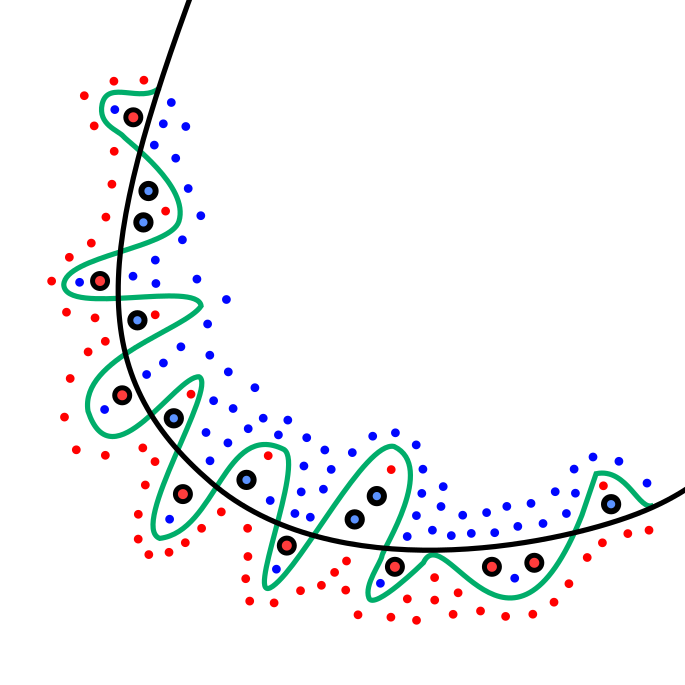
\includegraphics[width=0.5\linewidth]{images/overfitting.png}
    \caption{Due modelli (verde e nero) in un problema di classificazione binaria. Fonte: Chabacano, CC BY-SA 4.0 [https://creativecommons.org/licenses/by-sa/4.0].}
    \label{fig:overfitting}
\end{figure}

La Figura \ref{fig:overfitting} illustra un problema di classificazione binaria. Ciascuna osservazione corrisponde a un punto nel piano, che può appartenere alla classe blu oppure alla classe rossa. Si vuole quindi giungere a un classificatore in grado di predire, data un'osservazione, la classe di appartenenza. In questo caso, un classificatore non è altro che una funzione a due variabili, e l'obiettivo è trovare quella che meglio separa i punti blu da quelli rossi. Nella Figura \ref{fig:overfitting} ne sono illustrate due: una nera, che chiamiamo $\gamma$ e una verde, $\phi$.\\
I punti non contornati sono quelli utilizzati dall'algoritmo di addestramento, e fanno quindi parte del cosiddetto \textit{train set}, che indichiamo con $A$. I punti contornati, invece, rappresentano istanze nuove, non incontrate durante l'allenamento.

Chiaramente, la curva ideale sarebbe $\gamma$, che separa discretamente bene le osservazioni appartenenti a $A$ e perfettamente quelle nuove. Di certo, non potremmo affermare che $\phi$ sia un buon modello, in quanto non classifica correttamente neanche una delle osservazioni nuove. Eppure, se lo valutassimo solo su $A$, otterrebbe risultati migliori rispetto a $\gamma$. Quello esemplificato da $\phi$ è un fenomeno ben noto, chiamato \textit{overfitting}, dal quale ci si deve guardare in qualsiasi problema di ML. Infatti, $\phi$ si è specializzato eccessivamente su $A$, adattandosi alle caratteristiche peculiari dei suoi esempi che non avevano niente a che vedere con la relazione generale sottostante ai dati, e dunque non è in grado di \textit{generalizzare} su dati mai visti (cosa che $\gamma$ è in grado di fare).\\
Per questa ragione, valutare le performance di un modello solamente sul train set non basta per comprenderne la bontà: bisogna ricorrere a un \textit{test set} $T$, cioè un insieme di dati disgiunto da $A$.

Nonostante buone prestazioni sul train set non implichino la qualità del modello, rappresentano comunque una condizione necessaria per raggiungerla. Infatti, prestazioni scarse su $A$ indicano che il modello utilizzato non è abbastanza espressivo/potente per il dato problema (fenomeno di \textit{underfitting}). \\
Considerando nuovamente l'esempio della Figura \ref{fig:overfitting}, una retta rappresenterebbe un modello troppo poco espressivo per i dati presenti (nessuna funzione lineare separerebbe efficacemente i punti blu da quelli rossi), e soffrirebbe dunque di underfitting. Di fatto, avrebbe certamente prestazioni molto scarse già sul train set e a maggior ragione sul test set.

Nel Paragrafo \ref{par:tecniche-di-stima} presenteremo alcune tecniche con cui è possibile ricavare, a partire da un dataset, un train set e un test set disgiunto da esso.

\subsection{Tecniche di Stima delle Prestazioni}
\label{par:tecniche-di-stima}
Per quanto visto nel paragrafo precedente, è opportuno suddividere il dataset iniziale $D = \{(\mathbf{x}_1, y_1), \dots, (\mathbf{x}_n, y_n)\}$ in un train set $A$ e un test set $T$, garantendone la disgiunzione. \\
È fondamentale anche che entrambi $A$ e $T$ mantengano la distribuzione di $D$, poiché quest'ultimo rappresenta un campione della popolazione e, di conseguenza, ne rispecchia il profilo statistico (dovrebbe sempre farlo). Le tecniche di \textit{campionamento stratificato} servono proprio a fare in modo che qualsiasi sottoinsieme ricavato da $D$ ne rifletta la distribuzione. \\
Se $A$ e $T$ avessero distribuzioni diverse, staremmo valutando il modello su una popolazione distribuita diversamente rispetto a quella su cui è stato allenato. 

Prendiamo come esempio un problema di classificazione binaria. Supponiamo di avere $D$ contenente 500 esempi positivi e 500 esempi negativi, e di volerlo partizionare (tecnica che prende il nome di \textit{holdout}, come vedremo tra breve) in un train set $A$ con il 70\% degli esempi e un test set $T$ con il 30\% degli esempi. In tal caso, un metodo di campionamento stratificato garantirà che $A$ contenga 350 esempi positivi e 350 esempi negativi, e che $T$ contenga 150 esempi positivi e 150 esempi negativi.

Assumeremo sempre che qualsiasi sottoinsieme ricavato da $D$ sia correttamente stratificato.

\subsubsection{Holdout}
Come già accennato, la metodologia holdout consiste nell'approccio più intuitivo possibile: partizionare $D$, ossia nel suddividerlo in un train set $A$ e in un test set $T$, in modo tale che $D = T \cup A $ e $ T \cap A = \emptyset$. Nella Figura \ref{fig:holdout} è presente una visualizzazione grafica di questa metodologia.

\begin{figure}[h]
    \centering
    \begin{center}
    \begin{tikzpicture}
        \draw[thick] (0,3) rectangle (6,3.5);
        \node at (3,3.25) {\textbf{$D$}};

        \draw[thick,->] (3,2.8) -- (3,2.2);

        \draw[thick] (0,1.5) rectangle (6,2);
        \draw[thick] (4,1.5) -- (4,2);

        \node at (2,1.75) {\textbf{$A$}};
        \node at (5,1.75) {\textbf{$T$}};
    \end{tikzpicture}
\end{center}
    \caption{Visualizzazione grafica del metodo holdout.}
    \label{fig:holdout}
\end{figure}

Chiaramente, è necessario scegliere quanti degli esempi di $D$ inserire in $A$ e, di conseguenza, quanti in $T$. Di fatto, il rapporto $|A|/|D|$, e quindi $|T|/|D|$, è un aspetto critico del metodo holdout.
Aumentando la dimensione di $A$, le prestazioni del modello dovrebbero migliorare; tuttavia, la conseguente riduzione di $T$ porterebbe a un maggior errore nella stima della bontà di generalizzazione. Viceversa, aumentando la dimensione di $T$, la valutazione delle prestazioni sarebbe più accurata, ma la qualità delle risposte del modello ne risentirebbe.
Non esiste una soluzione perfetta a questo dilemma; è necessario un compromesso. Una pratica comune è
scegliere $|A|/|D| = 2/3$ oppure $|A|/|D| = 4/5$.

Mantenendo invariato il numero di esempi in $A$ (e di conseguenza in $T$), è possibile generare più coppie $(A,T)$ a partire dallo stesso dataset $D$, permutando gli esempi in modo casuale (curando sempre la stratificazione). In pratica, si eseguono $n$ holdout \textit{ripetuti} (ad esempio, 100), allenando e valutando altrettanti modelli, ciascuno su una coppia $(A,T)$ distinta, sempre derivata da $D$. \\
Per ottenere una valutazione complessiva, si calcola la media delle $n$ valutazioni ottenute. 

Successivamente, se la valutazione complessiva ottenuta è soddisfacente, si utilizza come train set l'intero dataset $D$ per ri-addestrare un ultimo modello, quello definitivo che verrà effettivamente impiegato. L'assunzione di fondo, generalmente corretta, è che allenando un modello con più dati, le sue prestazioni migliorino (o che sicuramente non peggiorino). L'operazione di \textit{ri-allenamento} finale svolta sull'intero dataset prende il nome di \textit{refit}, e viene sempre svolta, ammesso che la valutazione finale sia sufficientemente buona.

\subsubsection{Cross-validation}
La metodologia cross-validation (CV) (\cite{stone1974cross}) prevede di suddividere $ D $ in $ k $ sottoinsiemi di cardinalità uguale o simile, tali che 
\begin{equation}
    \begin{cases}
        D = \bigcup_{i=1}^{k} D_i \\
        D_i \cap D_j = \emptyset \quad \forall i, j \in \{1, \dots, k\}, \; i \neq j \enspace .
    \end{cases}
\end{equation}
In altre parole, i $k$ sottoinsiemi devono costituire una partizione di $D$.

Si effettuano $k$ iterazioni; a ogni iterazione, uno dei sottoinsiemi $D_i$ non ancora utilizzato come test set viene selezionato a tale scopo, mentre tutti i rimanenti sottoinsiemi vanno a costituire il training set, come illustrato in Figura \ref{fig:cross-validation}.  

Al termine delle iterazioni, si dispone di $k$ valutazioni, la cui media rappresenta la valutazione complessiva.  

Dal momento che la stabilità e l'accuratezza della CV dipendono fortemente dal valore di $k$, questa tecnica è nota anche come \textit{$k$-fold cross-validation}. Alcuni valori comuni per $k$ sono 3, 5 e 10.

\begin{figure}[h]
    \centering
    \begin{center}
    \begin{tikzpicture}
        \draw[thick] (0,6) rectangle (6,6.5);
        \node at (3,6.25) {$D$};

        \draw[thick,->] (3,5.8) -- (3,5.2);

        \foreach \y in {4.5,3.7,2.9,2.1,1.3} {
            \draw[thick] (0,\y) rectangle (6,\y+0.5);
        }

        \draw (4.8,4.5) rectangle (6,5);
        \draw (3.6,3.7) rectangle (4.8,4.2);
        \draw (2.4,2.9) rectangle (3.6,3.4);
        \draw (1.2,2.1) rectangle (2.4,2.6);
        \draw (0,1.3) rectangle (1.2,1.8);

        \node at (5.4,4.75) {$T_1$};
        \node at (4.2,3.95) {$T_2$};
        \node at (3,3.15) {$T_3$};
        \node at (1.8,2.35) {$T_4$};
        \node at (0.6,1.55) {$T_5$};

    \end{tikzpicture}
    \end{center}
    \caption{Una visualizzazione delle 5 suddivisioni diverse che si ottengono nella 5-fold CV.}
    \label{fig:cross-validation}
\end{figure}

L'intero processo di $k$-fold CV può essere ripetuto $p$ volte, permutando a ogni iterazione gli esempi di $D$ in maniera casuale per ridurre la dipendenza della valutazione dalla specifica suddivisione iniziale del dataset. Al termine delle iterazioni, si restituisce la media delle $p$ valutazioni ottenute. Un caso possibile è la \textit{10-times 10-fold CV}.

Una tipologia speciale di CV è la \textit{Leave-One-Out} (LOO), in cui si fissa $k = |D|$. Le valutazioni che ne risultano sono molto accurate, ma il costo computazionale dell'addestramento di $|D|$ modelli può essere proibitivo per dataset di grandi dimensioni.


\subsection{Tuning degli Iperparametri}
Mentre per i parametri di un modello i valori ottimali vengono definiti dall'algoritmo di addestramento, per gli iperparametri (vedi Paragrafo \ref{par:tassonomia}) è necessaria una apposita fase di \textit{tuning} (\cite{feurer2019hpo}). 

Di seguito, illustriamo un approccio molto diffuso per via della sua semplicità, che prende il nome di \textit{grid search}.

Consideriamo un modello avente $h$ iperparametri, con indice $i \in \{1,2, \dots, h \}$. Per ciascun iperparametro $i$, fissiamo un insieme di $v_i$ valori con cui sperimentare. È fondamentale scegliere con cura tali valori per evitare che il numero totale di combinazioni da esaminare, che indichiamo con $C$, cresca eccessivamente. Infatti, si ha:
\begin{equation}
    C = \prod_{i=1}^h v_i \enspace .
\end{equation}
Per ogni combinazione, si addestra e si valuta un modello; si sceglie poi quello con la performance migliore. Indichiamo con $c^*$ la combinazione di tale modello.

Come già discusso nel Paragrafo \ref{par:overfitting-underfitting}, non possiamo misurare le prestazioni limitandoci ad $A$. Dunque, per scegliere il modello migliore tra i $C$ generati, ricorriamo a un apposito \textit{validation set} $V$, ricavato da $D$ ma disgiunto da $A$ e da $T$.
Viene poi generato un modello $m$ con la combinazione $c^*$, allenandolo sull'unione $A \cup V$ (primo refit).  
Infine, si utilizza un apposito test set $T$ per valutare le performance di $m$. Se sono soddisfacenti, si effettua un secondo refit su $A \cup V \cup T$, ossia su $D$.

Un altro approccio possibile consiste nella \textit{random search}, che si basa su una ricerca casuale nello spazio delle combinazioni possibili (\cite{bergstra2012random}).

Nel Paragrafo \ref{par:tecniche-di-stima} abbiamo illustrato come valutare le prestazioni di un modello suddividendo il dataset $D$ nei sottoinsiemi $A$ e $T$. Tuttavia, non abbiamo considerato il caso in cui sia necessario eseguire il tuning degli iperparametri, introducendo quindi un ulteriore sottoinsieme, $V$.  

In questo scenario, le suddivisioni seguono una struttura annidata: una prima suddivisione esterna separa $D$ in $A$ e $T$, mentre una successiva suddivisione interna suddivide $A$ in un sottoinsieme di training ridotto e in $V$.  
Queste operazioni possono essere effettuate con lo stesso metodo (ad esempio, holdout-holdout), oppure con tecniche differenti, come nel caso di holdout seguito da CV. La Figura \ref{fig:cv-annidata} illustra una visualizzazione di quest'ultimo approccio.

\begin{figure}[h]
    \centering
    \begin{center}
    \begin{tikzpicture}
        \draw[thick] (0,7.5) rectangle (8, 8);
        \node at (4,7.75) {$D$};
        \draw[thick,->] (4,7.3) -- (4,6.7);
     
        \draw[thick] (0,6) rectangle (8,6.5);
        \node at (3,6.25) {$A$};
        \draw (6,6) -- (6,6.5);
        \node at (7,6.25) {$T$};

        \draw[thick,->] (3,5.8) -- (3,5.2);

        \foreach \y in {4.5,3.7,2.9,2.1,1.3} {
            \draw[thick] (0,\y) rectangle (6,\y+0.5);
        }

        \draw (4.8,4.5) rectangle (6,5);
        \draw (3.6,3.7) rectangle (4.8,4.2);
        \draw (2.4,2.9) rectangle (3.6,3.4);
        \draw (1.2,2.1) rectangle (2.4,2.6);
        \draw (0,1.3) rectangle (1.2,1.8);

        \node at (5.4,4.75) {$V_1$};
        \node at (4.2,3.95) {$V_2$};
        \node at (3,3.15) {$V_3$};
        \node at (1.8,2.35) {$V_4$};
        \node at (0.6,1.55) {$V_5$};

    \end{tikzpicture}
\end{center}
    \caption{In questo esempio, ciascuna configurazione di iperparametri viene valutata con una 5-fold CV annidata svolta su $A$, mentre la valutazione finale del modello viene effettuata su un test set esterno $T$ ricavato da $D$ tramite holdout.}
    \label{fig:cv-annidata}
\end{figure}

Un caso di particolare interesse si verifica quando la cross-validation viene utilizzata per la suddivisione esterna. A ciascuna iterazione esterna corrisponde un train set distinto, il che implica l'addestramento di un modello differente, con iperparametri ottimali che possono variare rispetto a quelli ottenuti nelle altre iterazioni. Di conseguenza, ogni iterazione esterna può generare un modello con una configurazione di iperparametri unica. In questo scenario, il modello finale può essere selezionato casualmente tra quelli addestrati.








\section{Tipologie di Modello}
\label{par:tipologie}
Presentiamo brevemente le famiglie di modelli di cui ci serviremo nei capitoli successivi.

\subsection{Support Vector Machine Lineari}
\label{par:svm}
Le Support Vector Machine (SVM) sono state proposte da \textcite{cortes1995svm} come una classe di algoritmi di apprendimento automatico utilizzabili principalmente per problemi di classificazione e di regressione. L'idea centrale delle SVM è quella di identificare un iperpiano ottimale che separi le istanze di dati appartenenti a classi differenti. \\
In questo paragrafo ci concentriamo sulle SVM lineari nel contesto della classificazione binaria.

Sia $D$ un dataset composto da $n$ esempi:
\begin{equation}
    D = \{ (\mathbf{x}_i, y_i) \in \mathbb{R}^d \times \{-1,+1 \}, \enspace i \in \{1,2, \dots, n \} \}.
\end{equation}
Ciascuna osservazione $\mathbf{x}_i$ è un vettore in $\mathbb{R}^d$ che rappresenta un punto in uno spazio a $d$ dimensioni, 
mentre $y_i$ è l’etichetta associata all’istanza, appartenente all’insieme $\{-1, +1\}$. Siamo quindi in un contesto di classificazione binaria.

L'idea di base è trovare nello spazio delle osservazioni un iperpiano in grado di separare istanze di classi diverse (se possibile, ossia se le istanze sono \textit{linearmente separabili}). Di iperpiani con questa caratteristica ce ne sono infiniti, per via della continuità di $\mathbb{R}^d$. Tuttavia, noi desideriamo quello più tollerante a piccole perturbazioni nei dati, ossia quello con la maggior capacità di generalizzazione. 

Facendo riferimento all'esempio bidimensionale della Figura \ref{fig:hyperplanes}, l'iperpiano (in questo caso, la retta) ideale sarebbe $H_1$, in quanto è poco probabile che piccole variazioni nelle posizioni delle osservazioni compromettano la correttezza della classificazione. $H_1$, oltre a separare correttamente le istanze in base alla classe, si mantiene alla massima distanza possibile da qualsiasi punto. Questo lo rende l'iperpiano ottimale. Al contrario, $H_2$ è molto suscettibile a piccole fluttuazioni delle osservazioni, in quanto vi si mantiene vicino.

\begin{figure}[ht]
    \centering
    \begin{tikzpicture}[scale=1.3]
    
        \draw[->] (-0.5,0) -- (4,0) node[right] {$x_1$};
        \draw[->] (0,-0.5) -- (0,4) node[above] {$x_2$};
    
        \foreach \x/\y in {0.3/2.8, 0.5/2.5, 1/2.6, 1.3/2.2, 1.5/2.4} {
            \filldraw[black] (\x,\y) circle (2pt);
        }
        
        \foreach \x/\y in {2/1, 2.3/0.7, 2.5/1.2, 3/1.5, 3.3/1.1} {
            \draw[black] (\x,\y) circle (2pt);
        }
    
        \draw[blue, thick] (1.75,-0.5) -- (1.75,4) node[above left] {$H_2$};
    
        \draw[red, thick] (-0.5,-0.5) -- (3.5,3.5) node[below right] {$H_1$};
    
        \node at (0.8,3.2) {$+1$};
        \node at (2.9,0.5) {$-1$};

    \end{tikzpicture}
    \caption{Un problema di classificazione binaria bidimensionale, con due possibili rette separatrici, $H_1$ e $H_2$.}
    \label{fig:hyperplanes}
\end{figure}

Se le osservazioni sono linearmente separabili, possiamo trovare due iperpiani paralleli $H^+$ e $H^-$ che separino correttamente le due classi, in modo tale che la distanza tra essi sia massima. L'iperpiano ottimale giace esattamente a metà tra $H^+$ e $H^-$. \\
La Figura \ref{fig:svm-margin} aiuta a visualizzare tutti e tre gli iperpiani di cui sopra con un esempio bidimensionale.

Possiamo descrivere i due iperpiani $H^+$ e $H^-$ con le seguenti equazioni: 

\begin{equation}
    \begin{aligned}
        H^+ &: \mathbf{w}^{\top} \mathbf{x}+b=+1 \\
        H^- &: \mathbf{w}^{\top} \mathbf{x}+b=-1 \enspace .
    \end{aligned}
\end{equation}

Stiamo dunque chiedendo che, per qualsiasi esempio $(\mathbf{x}_i, y_i) \in D$, valga:

\begin{equation}
    \begin{cases}
        \mathbf{w}^{\top} \mathbf{x}_i +b \geq +1, \quad \text{se } y_i=+1, \\
        \mathbf{w}^{\top} \mathbf{x}_i +b \leq -1, \quad \text{se }y_i=-1 \enspace .
    \end{cases}
\end{equation}
Possiamo sintetizzare questi vincoli imponendo
\begin{equation}
    y_i(\mathbf{w}^{\top} \mathbf{x}_i +b) \geq 1, \quad \forall \space i \in \{1, \dots, n\} \enspace .
\end{equation}

La distanza tra $H^+$ e $H^-$, nota come \textit{margine}, può essere espressa come
\begin{equation}
    \frac{2}{\|\mathbf{w}\|} \enspace ,
\end{equation}
ed è proprio la quantità che vogliamo massimizzare.

\begin{figure}[ht]
    \centering
    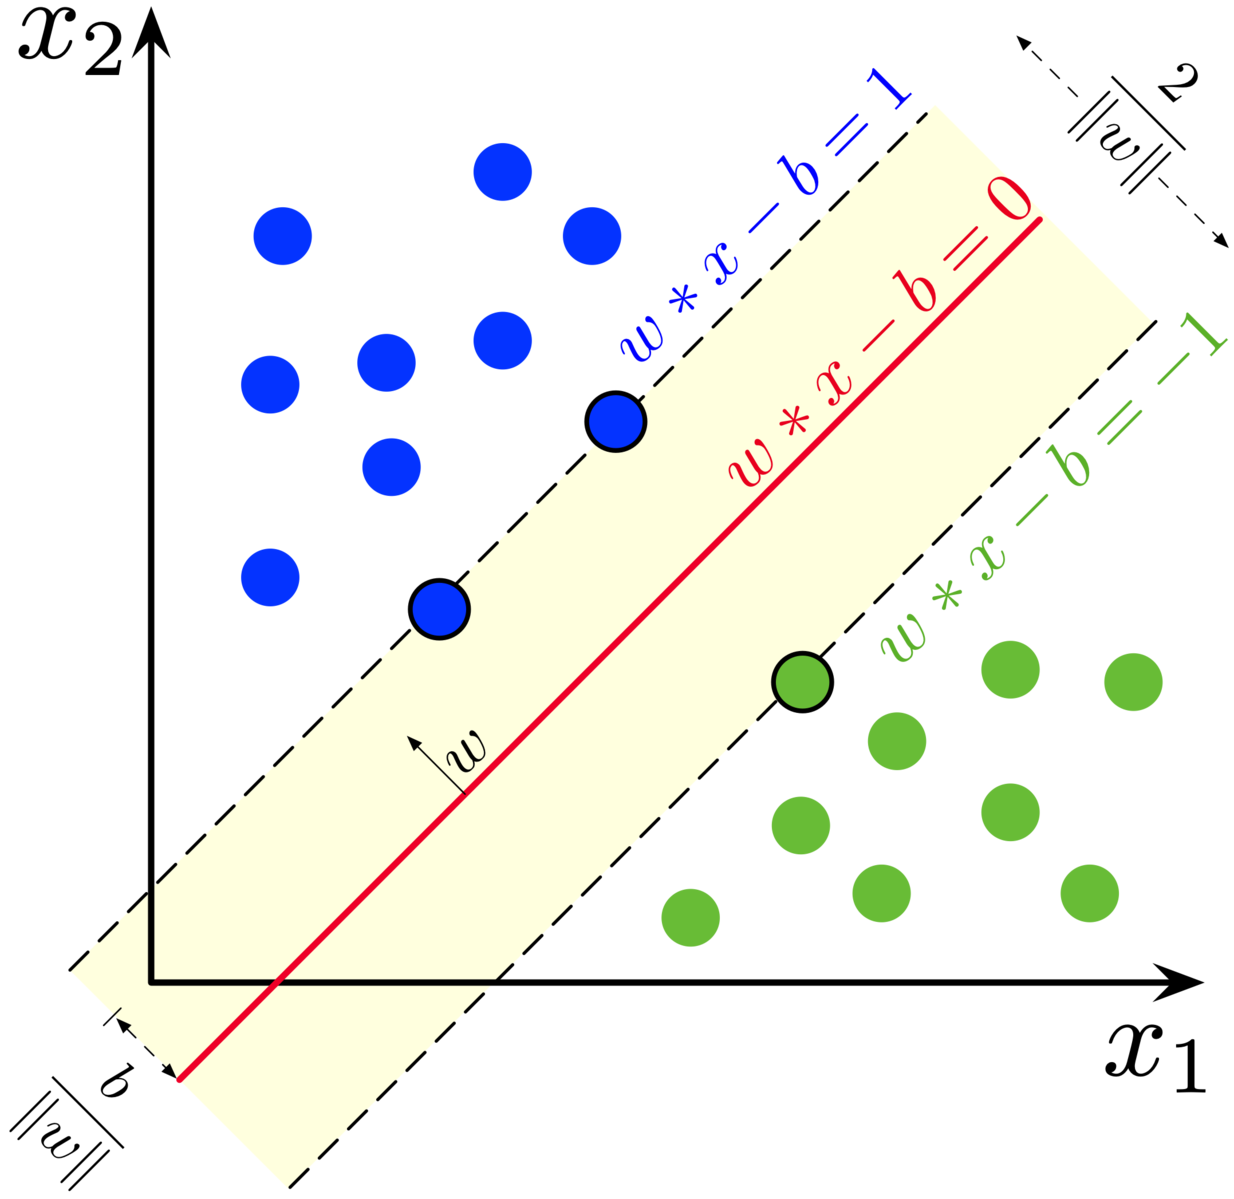
\includegraphics[width=0.5\linewidth]{images/svm-margin.png}
    \caption{I due iperpiani (rette) di margine massimo e l'iperpiano separatore che vi giace in mezzo. In questo esempio, $b$ è preceduto da un segno negativo, diversamente da quanto scritto finora; si tratta di formulazioni equivalenti. Fonte: Larhmam, CC BY-SA 4.0 [https://creativecommons.org/licenses/by-sa/4.0].}
    \label{fig:svm-margin}
\end{figure}

Tenuto conto che massimizzare $\|\mathbf{w}\|^{-1}$ equivale a minimizzare $\|\mathbf{w}\|^2$, possiamo scrivere il problema di ottimizzazione a cui siamo giunti in questo modo:
\begin{equation}
    \begin{aligned}
    \min_{\mathbf{w},b} \quad & \frac{1}{2}\|\mathbf{w}\|^2 \\
    \text{s.t.} \quad & y_i(\mathbf{w}^{\top} \mathbf{x}_i +b) \geq 1, \quad \forall \space i \in \{1, \dots, n\} \enspace .
    \end{aligned}
    \label{expr:primal-hard-margin}
\end{equation}

È importante notare che l'iperpiano separatore ottimale è completamente determinato dai punti $\mathbf{x}_i$ che si trovano più vicini a esso, come evidenziato in Figura \ref{fig:svm-margin}. Questi $\mathbf{x}_i$ sono chiamati \textit{support vector} (da cui il nome della famiglia di modelli).

Il problema di ottimizzazione vincolata (\ref{expr:primal-hard-margin}) riguarda il caso \textit{hard margin}, ossia quello in cui le osservazioni sono linearmente separabili. Comunemente, però, ciò non accade, e quindi si adotta un approccio \textit{soft margin}, nel quale si tollera che la SVM commetta qualche errore, permettendo la violazione del vincolo $y_i(\mathbf{w}^{\top} \mathbf{x}_i +b) \geq 1$ per qualche $i$.

A questo scopo, modifichiamo (\ref{expr:primal-hard-margin}) introducendo delle variabili \textit{di slack} $\xi_i$:
\begin{equation}
    \begin{aligned}
    \min_{\mathbf{w},b} \quad & \frac{1}{2}\|\mathbf{w}\|^2 + C \sum_{i=1}^n \xi_i \\
    \text{s.t.} \quad & y_i(\mathbf{w}^{\top} \mathbf{x}_i +b) \geq 1 - \xi_i, \\
    & \xi_i \geq 0, \quad \forall \space i \in \{1, \dots, n\} \enspace .
    \end{aligned}
    \label{expr:primal-soft-margin}
\end{equation}

Grazie a questa nuova formulazione, ciascuna $\xi_i$ vale più di 0 solo se l'osservazione $i$-esima vìola il vincolo $y_i(\mathbf{w}^{\top} \mathbf{x}_i +b) \geq 1$. Dunque, la somma di tutte le $\xi_i$ quantifica la violazione complessiva del suddetto vincolo. Penalizzando la funzione obiettivo originale in (\ref{expr:primal-hard-margin}) con questa somma, moltiplicata per una costante $C>0$ (che sarà un iperparametro), modelliamo il caso soft margin. All'aumentare di $C$, la penalizzazione pesa maggiormente sull'obiettivo; di conseguenza, la SVM tollera sempre meno gli errori.

Sfruttando i moltiplicatori di Lagrange, possiamo passare al \textit{problema duale} di (\ref{expr:primal-soft-margin}):
\begin{equation}
    \begin{aligned}
    \max_{\boldsymbol{\alpha}} \quad & \sum_{i=1}^{n} \alpha_i - \frac{1}{2} \sum_{i=1}^{n} \sum_{j=1}^{n} \alpha_i \alpha_j y_i y_j \mathbf{x}_i^{\top} \mathbf{x}_j \\
    \text{s.t.} \quad & \sum_{i=1}^{n} \alpha_i y_i = 0, \\
    & 0 \leq \alpha_i \leq C, \quad \forall \space i \in \{1, \dots, n\} \enspace .
    \end{aligned}
\end{equation}
Dal momento che si tratta di un problema di ottimizzazione non lineare vincolata, vanno soddisfatte le condizioni di Karush-Kuhn-Tucker (KKT):
\begin{equation}
        \begin{cases}
            \alpha_i \geq 0, \quad \mu_i \geq 0, \\
            y_i f(\mathbf{x}_i)-1 + \xi_i \geq 0, \\
            \alpha_i (y_i f(\mathbf{x}_i)-1 + \xi_i) = 0, \\
            \xi_i \geq 0, \quad \mu_i \xi_i = 0 \enspace ,
        \end{cases}
\end{equation}
dove $f(\mathbf{x}) = \mathbf{w}^{\top} \mathbf{x} +b$; ossia, $f(\mathbf{x})$ è l'espressione dell'iperpiano separatore.

Dalle KKT evinciamo che, per qualsiasi esempio $(\mathbf{x}_i, y_i) \in D$:
\begin{itemize}
    \item se $\alpha_i =0$, allora $y_i f(\mathbf{x}_i)-1 + \xi_i$ può assumere qualsiasi valore; in altre parole, l'esempio $i$-esimo non ha influenza sull'iperpiano.

    \item Se $\alpha_i > 0$, allora necessariamente si ha $y_i f(\mathbf{x}_i) = 1 -\xi_i$, ossia: $\mathbf{x}_i$ contribuisce a determinare l'iperpiano ed è quindi un support vector.
\end{itemize}

\subsubsection{Variante Cost-Sensitive}

Finora abbiamo considerato una SVM classica, che tratta gli errori in maniera omogenea, senza distinzione tra FP e FN.
Tuttavia, come vedremo nei prossimi capitoli, è di nostro interesse poter attribuire una gravità diversa ai FP rispetto che ai FN, per poter regolare il FPR e, di conseguenza, il FNR di una SVM (ricordiamo che, come sottolineato nel Paragrafo \ref{par:metriche}, FP e FN sono generalmente in mutua competizione). Infatti, ciò che si vuole ottenere è una SVM \textit{cost-sensitive} che tolleri più errori di un tipo (ad esempio, FP), ma meno dell'altro.

A tale scopo, un possibile approccio proposto da \textcite{morik:1999:svm} consiste nel separare la sommatoria della funzione obiettivo di (\ref{expr:primal-soft-margin}) per distinguere la penalizzazione dovuta ai FP da quella dovuta ai FN, e moltiplicare ciascuna per il proprio fattore di costo, rispettivamente $C_+$ e $C_-$ (questi ultimi sono a tutti gli effetti degli iperparametri). Si ottiene:
\begin{equation}
    \begin{aligned}
    \min_{\mathbf{w},b} \quad & \frac{1}{2}\|\mathbf{w}\|^2 + C_+ \sum_{i:y_i=+1}^n \xi_i + C_- \sum_{i:y_i=-1}^n \xi_i \\
    \text{s.t.} \quad & y_i(\mathbf{w}^{\top} \mathbf{x}_i +b) \geq 1 - \xi_i, \\
    & \xi_i \geq 0, \quad \forall \space i \in \{1, \dots, n\} \enspace .
    \end{aligned}
\end{equation}
Se $C_+ > C_-$, gli errori commessi sugli esempi positivi, ossia i FN, gravano maggiormente sull'obiettivo rispetto ai FP, dunque la SVM tenderà a commettere meno FN e più FP. Se, invece, $C_+ < C_-$, la SVM commetterà meno FP e più FN.
Il caso in cui $C_+ = C_-$ ci riporta al problema originale, in cui FP e FN hanno la stessa importanza.

Essenzialmente, $C_+ >0$ e $C_- >0$ hanno la stessa funzione dell'iperparametro $C$ introdotto nel caso non cost-sensitive, ma si occupano ciascuno di una delle due classi in maniera separata.









\subsection{Reti Neurali}
\label{par:nn}
Una rete neurale (\textit{Neural Net}, NN) è una tipologia di modello di ML ispirata alla struttura e al funzionamento del sistema nervoso centrale delle specie animali.

L'oggetto astratto alla base delle NN è il neurone artificiale (\cite{mcculloch1943}), schematizzato in Figura \ref{fig:neuron}. Ciascun neurone riceve uno o più input, ne effettua la somma pesata, ci aggiunge un termine costante $b$ noto come \textit{bias}, e sottopone il risultato a una \textit{funzione di attivazione} $\alpha$ per ottenere l'output $y$:
\begin{equation}
    y = \alpha \left(\sum_{j=1}^d w_j x_j + b \right) \enspace ,
    \label{expr:neuron-output}
\end{equation}
dove $d$ è il numero di input (e di conseguenza di pesi).

\begin{figure}[ht]
    \centering
    \begin{tikzpicture}

    \node (x1) at (0,1.5) {$x_1$};
    \node (x2) at (0,0.5) {$x_2$};
    \node (xdots) at (0,-0.5) {$\vdots$};
    \node (xn) at (0,-1.5) {$x_d$};

    \node (w1) at (1,1.5) {$w_1$};
    \node (w2) at (1,0.5) {$w_2$};
    \node (wdots) at (1,-0.5) {$\vdots$};
    \node (wn) at (1,-1.5) {$w_d$};
    
    \node[draw, circle, minimum size=1cm] (sum) at (3,0) {$\sum$};

    \node (b) at (2,-2) {$b$};
    \draw[->] (b) -- (sum);

    \node[draw, rectangle, minimum width=1.2cm, minimum height=0.8cm] (act) at (5,0) {$\alpha$};

    \node (y) at (7,0) {$y$};

    \draw[->] (x1) -- (sum);
    \draw[->] (x2) -- (sum);
    \draw[->] (xn) -- (sum);
    
    \draw[->] (sum) -- (act);
    \draw[->] (act) -- (y);

\end{tikzpicture}
    \caption{Un neurone artificiale.}
    \label{fig:neuron}
\end{figure}

Una tipica funzione di attivazione è la sigmoide (il cui grafico è illustrato in Figura \ref{fig:sigmoid}):
\begin{equation}
    \alpha(x) = \frac{1}{1+e^{-x}} \enspace .
\end{equation}

\begin{figure}[ht]
    \centering
    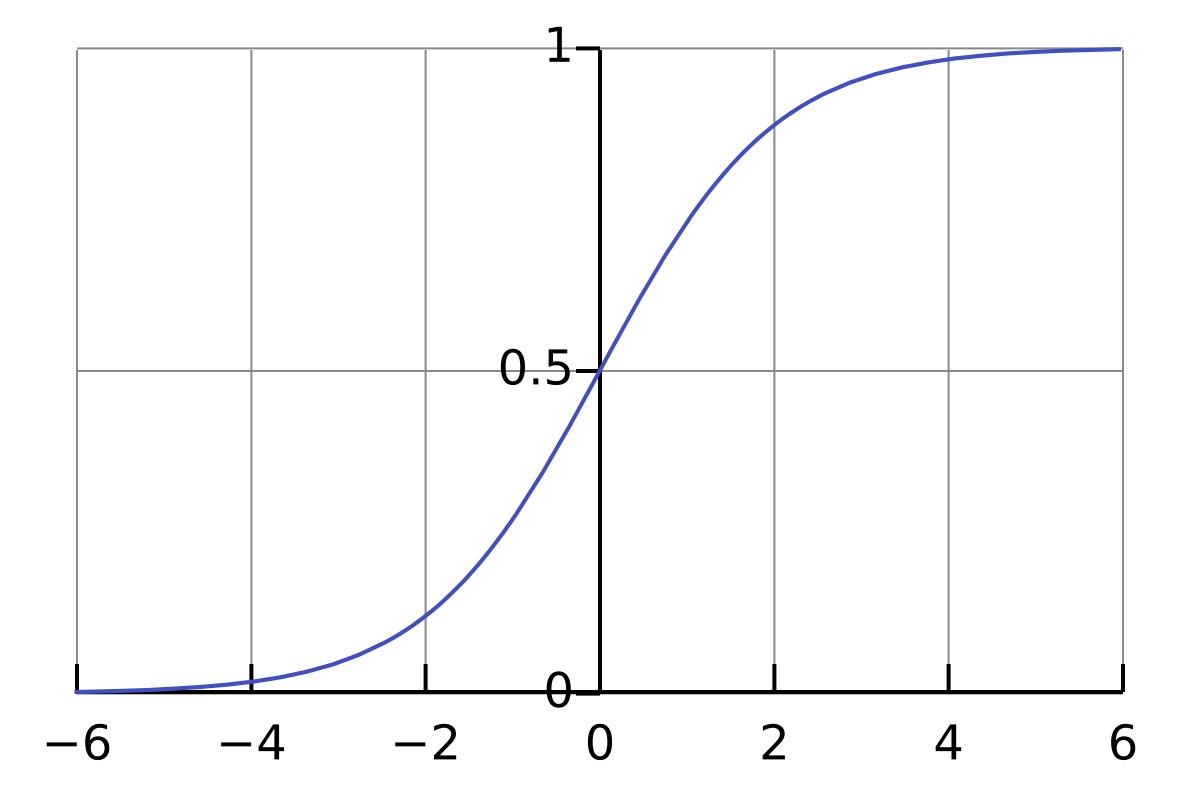
\includegraphics[width=0.5\linewidth]{images/sigmoid.png}
    \caption{La funzione sigmoide.}
    \label{fig:sigmoid}
\end{figure}

Più neuroni possono essere collegati a formare una NN come quella in Figura \ref{fig:neural-net} (\cite{zhou2021ml}). Si tratta di una tipica rete a più strati, in cui ogni neurone di ogni strato è connesso con tutti quelli dello strato successivo. I neuroni facenti parte dello stesso strato o di strati non adiacenti, invece, non sono connessi. NN di questo tipo prendono il nome di reti neurali multistrato \textit{feedforward}, perché l'informazione, durante la classificazione di un'istanza, viaggia solamente \textit{in avanti}: partendo dallo strato di input, attraversa uno a uno gli strati nascosti per poi giungere allo strato di output. Quest'ultimo, in un problema di classificazione binaria, è composto da un solo neurone, il cui output è un valore $o$ nell'intervallo continuo $[0,1]$. Tale valore viene confrontato con una soglia $\tau \in [0,1]$: l'osservazione $\mathbf{x}$ viene classificata come positiva se e solo se $o_{\mathbf{x}} > \tau$.

Ciascun neurone si comporta allo stesso modo, producendo un output secondo (\ref{expr:neuron-output}). \\
Per la precisione, lo strato di input non è composto da neuroni: ogni nodo rappresenta semplicemente un attributo dell'osservazione, il cui valore va direttamente in input allo strato successivo.

\begin{figure}[h]
    \centering
    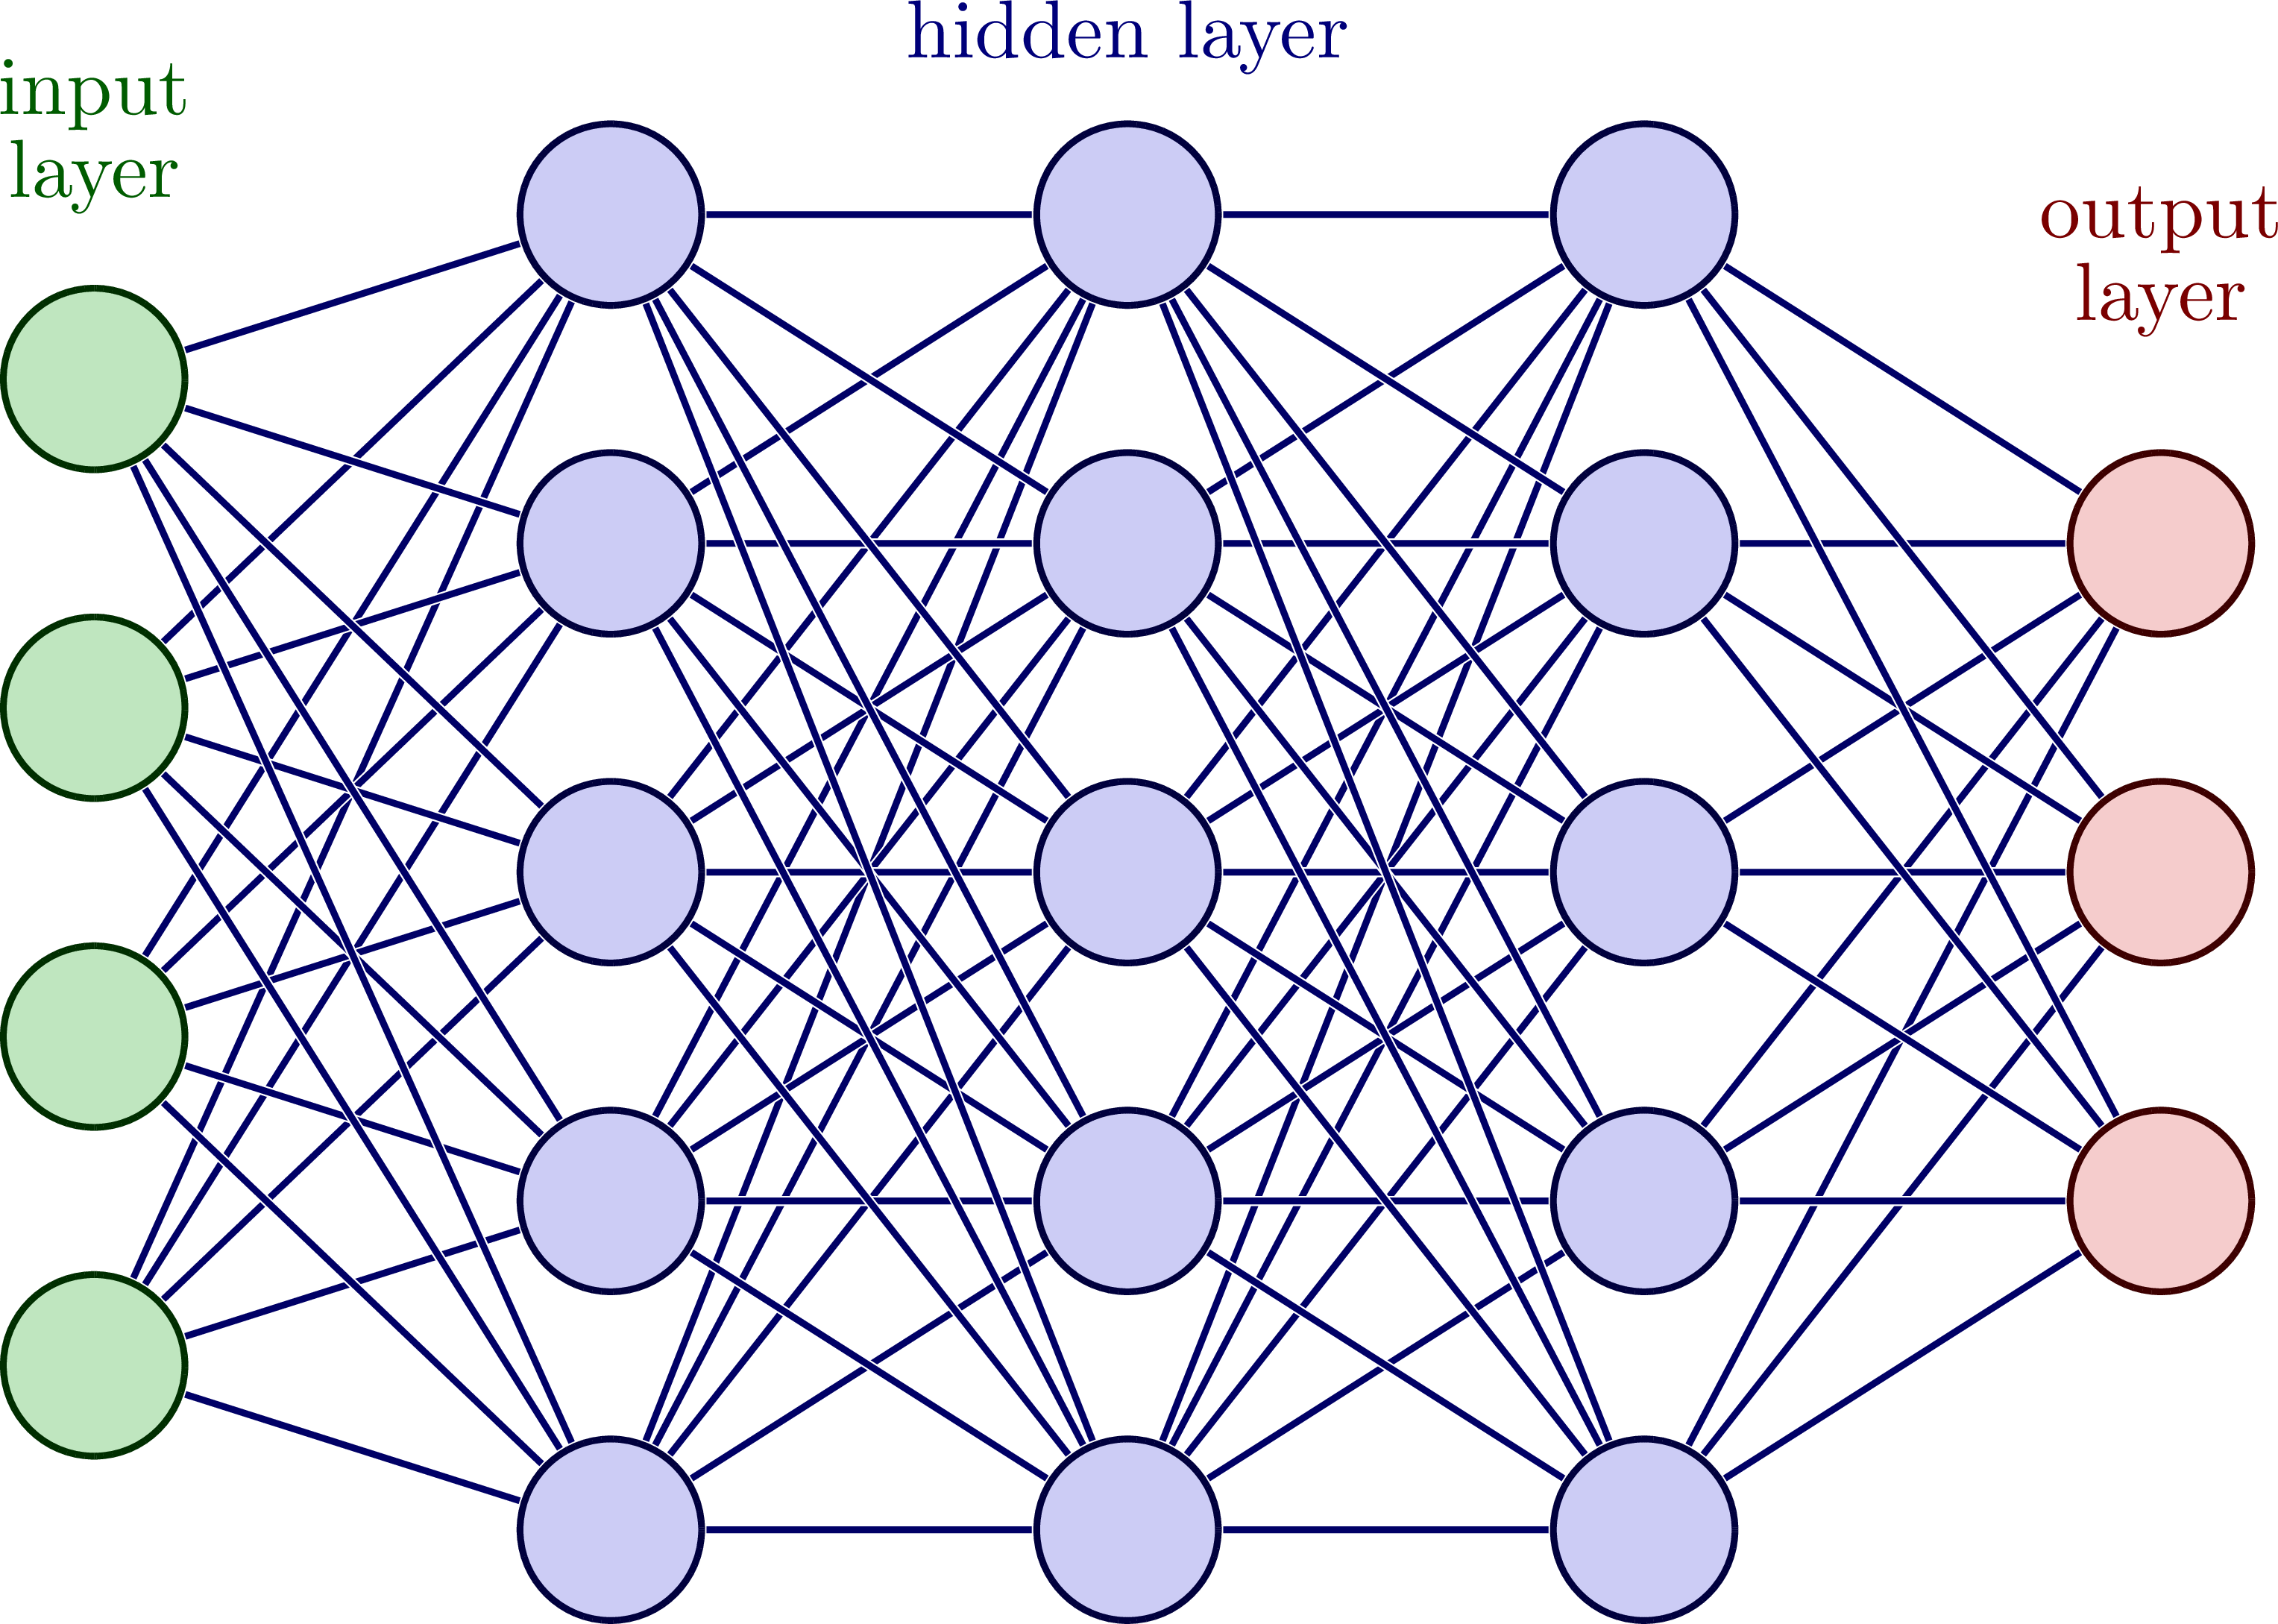
\includegraphics[width=0.6\linewidth]{images/neural-net.png}
    \caption{Una rete neurale \textit{feedforward}. Fonte: Izaak Neutelings, CC BY-SA 4.0 [https://creativecommons.org/licenses/by-sa/4.0].}
    \label{fig:neural-net}
\end{figure}

L'algoritmo di apprendimento delle NN ha come scopo trovare i valori ottimali dei pesi e dei bias, che sono quindi i parametri di questa tipologia di modello. Tale algoritmo si basa su una \textit{funzione di perdita} $L$ (dall'inglese \textit{loss}), che misura la discrepanza tra le previsioni del modello e i valori reali.

Una funzione comunemente utilizzata è l'errore quadratico medio (MSE), che per l'esempio $i$-esimo è definita come:
\begin{equation}
    L_i = \frac{1}{2} \sum_{k=1}^l (y_k^i - \hat{y}_k^i)^2
\end{equation}
dove $l$ è il numero di neuroni di output, $y_k^i$ è il valore che il $k$-esimo neurone di output dovrebbe restituire (facilmente ricavabile dall'etichetta $i$-esima) e $\hat{y}_k^i$ è il valore effettivo che tale neurone restituisce.

Da notare che ogni $L_i$ è in realtà una funzione dei pesi e dei bias della rete, in quanto sono questi a determinare ciascun $\hat{y}_k^i$. Quindi, per ciascun esempio, basterebbe calcolare il gradiente $\nabla L_i$, che ci dà la direzione di massimizzazione di $L_i$, e aggiornare i pesi e i bias della rete per muoversi nella direzione opposta. Questa è l'idea alla base dell'algoritmo di apprendimento delle NN, anche se quest'ultimo opera in realtà in maniera particolare, sfruttando la struttura e il funzionamento della rete.

Per minimizzare $L_i$, funzione che spesso dipende da un elevato numero di variabili, il gradiente viene calcolato iterativamente attraverso un processo noto come \textit{backpropagation} (\cite{hinton1986backpropagation}). L'idea alla base di questo metodo è che la derivata parziale di $L_i$ rispetto a un peso/bias in uno strato qualsiasi può essere ottenuta sfruttando le derivate parziali rispetto ai pesi degli strati successivi, applicando la regola della catena. In altre parole, l’influenza sulla funzione di perdita di un peso nel primo strato è indiretta: passa necessariamente attraverso i pesi degli strati successivi, fino all’ultimo strato.

Questo procedimento si configura come un algoritmo di \textit{programmazione dinamica}: ogni derivata viene calcolata una sola volta, partendo da quelle che non dipendono da altre, ossia quelle relative all'ultimo strato, e muovendosi a ritroso nella rete utilizzando queste ultime per calcolare tutte le altre a cascata.

Appena si ottiene una derivata parziale, è possibile aggiornare il peso (o il bias) corrispondente secondo la regola di discesa del gradiente:  

\begin{equation}
    w_h \leftarrow w_h - \eta \frac{\partial L_i}{\partial w_h}
\end{equation}
dove $\eta > 0$ è il tasso di apprendimento (\textit{learning rate}), parametro che regola l’entità della variazione dei pesi a ogni aggiornamento.

Un grande vantaggio delle NN è il fatto di poter stabilire la topologia di rete (che è a tutti gli effetti un iperparametro): le NN possono raggiungere dimensioni dell'ordine di miliardi di parametri, modellando problemi complessi, oppure possono, con pochi neuroni, comportarsi bene in problemi più semplici non risolvibili da modelli lineari come le SVM.

Un altro iperparametro rilevante per la nostra discussione è il numero di \textit{epoche}, $E$, che rappresenta il numero di volte in cui l'intero train set viene sottoposto al modello durante l'addestramento. Possiamo vedere $E$ come una misura di quanto la rete deve apprendere dal train set. Se $E$ è troppo basso, il modello non si adatta sufficientemente ai dati forniti, andando incontro a una situazione di underfitting; al contrario, se $E$ è troppo alto, il modello si specializza eccessivamente sul train set e dunque si verifica overfitting.

\subsubsection{Variante Cost-Sensitive}
Come per le SVM (Paragrafo \ref{par:svm}), anche per le NN la variante cost-sensitive è di nostro interesse.
Un possibile modo di ottenere una NN di questo tipo è attribuendo a ciascun esempio del dataset un peso, che dipende esclusivamente dalla classe a cui appartiene, e che va a influenzare direttamente la funzione di perdita $L$.

Abbiamo visto un caso specifico di questa funzione, che adotta il MSE, per un singolo esempio. Ora, generalizziamo $L$ per renderla indipendente dal tipo specifico di errore misurato, e mediamo su tutti gli esempi di un insieme \textit{batch} $B$ per ottenere $L$ e non più $L_i$. Inoltre, indichiamo con $W$ una generica combinazione di valori per tutti i parametri della rete (pesi e bias); fissata la topologia, $W$ rappresenta l'interezza della rete. Allora, possiamo scrivere:
\begin{equation}
    L(W)= \frac{1}{|B|} \sum_{(\mathbf{x}_i, y_i) \in B} \text{err}(W,(\mathbf{x}_i, y_i)) \enspace ,
\end{equation}
dove $\text{err}(W,(\mathbf{x}_i, y_i))$ rappresenta l'errore, calcolato in un generico modo, che la rete $W$ commette quando sottoposta all'esempio $(\mathbf{x}_i, y_i)$.
Come abbiamo già discusso, ciò che ci interessa è calcolare il gradiente di $L$. Considerando un generico parametro $w$ della rete, e applicando la proprietà secondo cui la derivata della somma è la somma delle derivate, otteniamo
\begin{equation}
    \frac{\partial L}{\partial w} = \frac{1}{|B|} \sum_{(\mathbf{x}_i, y_i) \in B} \frac{\partial \text{err}(W,(\mathbf{x}_i, y_i))}{\partial w} \enspace .
\end{equation}

Associamo ora, a ogni esempio $(\mathbf{x}_i, y_i) \in B$, un valore $\nu_i$ che indica il peso dell'esempio stesso in $L$:
\begin{equation}
    L(W)= \frac{1}{|B|} \sum_{(\mathbf{x}_i, y_i) \in B} \nu_i \cdot \text{err}(W,(\mathbf{x}_i, y_i)) \enspace .
\end{equation}
Derivando, otteniamo
\begin{equation}
    \frac{\partial L}{\partial w} = \frac{1}{|B|} \sum_{(\mathbf{x}_i, y_i) \in B} \nu_i \cdot  \frac{\partial \text{err}(W,(\mathbf{x}_i, y_i))}{\partial w} \enspace .
\end{equation}

Chiaramente, dal momento che vogliamo poter attribuire più o meno importanza ai FP rispetto che ai FN, utilizzeremo lo stesso peso $C_+$ per tutti gli esempi positivi e lo stesso $C_-$ per quelli negativi. Dunque, $C_+$ e $C_-$ sono iperparametri che possiamo sfruttare in maniera analoga a quanto visto per le SVM.








\subsection{Alberi di Decisione}
\label{par:dt}
Un albero di decisione (\textit{decision tree}, DT) è un modello di classificazione organizzato come un albero in cui ogni nodo interno rappresenta una decisione basata sul valore di un attributo di un'osservazione, e le foglie rappresentano previsioni fatte per tale osservazione, ossia le classi (\cite{breiman1986dt}). Nella Figura \ref{fig:decision-tree} è raffigurato un semplice esempio di classificazione binaria mediante DT.

Un'osservazione $\mathbf{x}_i$, per essere classificata, segue un cammino che parte dalla radice e che segue di volta in volta il ramo relativo alla casistica in cui $\mathbf{x}_i$ rientra, terminando nella foglia con l'annessa predizione.

\begin{figure}[h]
    \centering
    \begin{forest}
    for tree={align=center, edge={->}, draw, rounded corners}
    [Età $\geq$ 18?
        [Reddito $\geq$ 30k?, edge label={node[midway, above, yshift=2pt, left]{\scriptsize Sì}}
            [Idoneo, edge label={node[midway, above, yshift=2pt, left]{\scriptsize Sì}}]
            [Età $\geq$ 25?, edge label={node[midway, above, yshift=2pt, right]{\scriptsize No}}
                [Idoneo, edge label={node[midway, above, yshift=2pt, left]{\scriptsize Sì}}]
                [Non idoneo, edge label={node[midway, above, yshift=2pt, right]{\scriptsize No}}]
            ]
        ]
        [Non idoneo, edge label={node[midway, above, yshift=2pt, right]{\scriptsize No}}]
    ]
    \end{forest}
    \caption{Un semplice albero di decisione per valutare se una persona è idonea o non idonea a ricevere un prestito, basato su età e reddito.}
    \label{fig:decision-tree}
\end{figure}


L’algoritmo di apprendimento produce, partendo dal train set, l'intero DT; deve quindi stabilirne la struttura, le condizioni presenti nei nodi interni e le classi nelle foglie.

Gli elementi chiave sono chiaramente i nodi di decisione, che devono essere i più efficaci possibili. Un nodo di decisione è tanto più efficace quanto più omogenee, in termini di classi, sono le osservazioni in ciascuno dei nodi figli. Infatti, il nodo ideale sarebbe quello che, partendo dall'intero train set, composto da esempi negativi e positivi, produrrebbe due nodi figli, uno contenente solo esempi positivi e l'altro solo esempi negativi. Tali nodi, in cui l'omogeneità è massima, diventano automaticamente foglie; non avrebbe senso cercare in essi criteri di decisione per separare le classi.
Questo nodo-utopia, nella realtà, non è ottenibile. Tuttavia, rappresenta un obiettivo a cui ogni nodo dell'albero deve tendere il più possibile.

Esistono varie misure di eterogeneità; una delle più utilizzate è l'\textit{indice di eterogeneità di Gini}. Restando nel caso specifico della classificazione binaria, di nostro interesse, supponiamo di avere un insieme $A$ di esempi in cui $f_+$ e $f_-$ sono rispettivamente la frequenza relativa degli esempi positivi e quella degli esempi negativi. L'indice di eterogeneità di Gini, in questo caso, è dato da:
\begin{equation}
    I(A) = 1- f_+^2 - f_-^2 \enspace ,
\end{equation}
ma può essere riscritto anche come
\begin{equation}
    I(A) = 2 f_+ (1 - f_+)
\end{equation}
sfruttando il fatto che $f_- = 1 - f_+$.

$I(A)$ vale 0 nel caso di minima eterogeneità (massima omogeneità), ossia quando $A$ contiene solo esempi positivi o solo esempi negativi; vale $\frac{1}{2}$ nel caso di massima eterogeneità (minima omogeneità), ossia quando $A$ è composto per metà da esempi positivi e per metà da esempi negativi.

Supponiamo di aver scelto un criterio di decisione $\delta$ basandoci su uno degli attributi, e che tale criterio generi $Q$ possibili casistiche. Il nodo associato a $\delta$ ha dunque $Q$ figli, e ciascun figlio ha a sua volta un insieme $A^q$ di esempi, quelli che rientrano nella casistica $q$.

Basandoci sull'indice di eterogeneità di Gini, possiamo definire una quantità $G(A,\delta)$ che misura l'eterogeneità complessiva portata dal criterio $\delta$ per l'insieme $A$:
\begin{equation}
    G(A,\delta) = \sum_{q=1}^Q \frac{|A^q|}{|A|} I(A^q) \enspace .
\end{equation}
Non è altro che la somma degli indici di eterogeneità dei sottoinsiemi ``figli" $A^q$ generati con $\delta$, pesati ciascuno per il numero di esempi che contiene rispetto all'insieme ``padre" $A$.

Dato un insieme $\Delta$ di criteri candidati, selezioniamo il criterio $\delta^*$ tale che:
\begin{equation}
    \delta^* = \arg \min_{\delta \in \Delta} G(A,\delta) \enspace ,
\end{equation}
ossia quello che minimizza $G(A,\delta)$.


L'idea principale dietro l'algoritmo di apprendimento di un DT è quindi quella di costruire ricorsivamente la struttura dell’albero, generando a ogni iterazione i figli di ciascuna foglia.
Per ciascun nodo, ragionando sull'insieme di dati a esso associato (per la radice è l'intero train set), si sceglie il criterio di decisione che minimizzi l'eterogeneità nei nodi figli.

Esistono delle condizioni d'arresto tali per cui una generica foglia $N$ non può generare figli. Le più comuni includono:
\begin{itemize}
    \item $N$ contiene una classe predominante, tale da rendere poco o per nulla significativa un'ulteriore suddivisione; 

    \item $N$ si trova alla profondità massima, definita come iperparametro;

    \item $N$ contiene un numero minimo di esempi (anch'esso iperparametro).
\end{itemize}
L'algoritmo di addestramento termina quando tutti i nodi foglia soddisfano almeno una delle condizioni di arresto. Se queste non sono sufficientemente stringenti, il DT può arrivare a suddividere i dati fino a ottenere gruppi perfettamente (o quasi) omogenei nei nodi foglia, adattandosi in maniera molto precisa al train set. Di fatto, questo tipo di modello si presta particolarmente bene all'overfitting.

\subsubsection{Variante Cost-Sensitive}
Illustriamo ora una variante cost-sensitive dei DT che si basa, come nel caso delle NN, sull'attribuire un peso ai singoli esempi del train set (\cite{ting2002dt}). Tale peso dipende, chiaramente, dalla classe a cui ciascun esempio appartiene. 

Con questa modifica, possiamo calcolare diversamente l'indice di omogeneità o di eterogeneità che abbiamo scelto di utilizzare, in modo tale che tenga conto dei pesi degli esempi. Sia $A$ l'insieme corrente, e siano $A_+, A_-$ rispettivamente il sottoinsieme degli esempi positivi e quello dei negativi. Definiamo $W_+$ come la somma dei pesi associati ai positivi:
\begin{equation}
    W_+ = w_+ |A_+| \enspace,
\end{equation}
dove $w_+$ è il peso attribuito a tutti i positivi. Analogamente, definiamo $W_-$:
\begin{equation}
    W_- = w_- |A_-| \enspace.
\end{equation}
Sia $f_+'$ il rapporto tra il peso totale degli esempi positivi e il peso complessivo degli esempi in $A$:
\begin{equation}
    f'_+ = \frac{W_+}{W_+ + W_-} \enspace.
\end{equation}
Possiamo ridefinire l'indice di eterogeneità di Gini sostituendo $f_+$ con $f_+'$, sfruttando così anche le informazioni relative ai pesi:
\begin{equation}
    I'(A) = 2f_+'(1-f_+') \enspace.
\end{equation}
Integrando questa modifica nell'algoritmo di addestramento di un DT, i criteri di decisione verranno scelti tenendo in considerazione i pesi degli esempi.

Ciò che si vuole definire, però, non è direttamente il peso da associare a ogni esempio positivo e quello da associare a ogni esempio negativo: vorremmo poter determinare degli iperparametri $C_+, C_-$ tali che, per qualsiasi insieme $A$ di esempi, producano un insieme di esempi pesati tale che $W_+ + W_- = |A|$. 
Dunque, definiti $C_+$ e $C_-$, automaticamente derivano $w_+$ e $w_-$. In particolare:
\begin{equation}
    \begin{aligned}
        w_+ &= C_+ \frac{|A|}{C_+|A_+| + C_-|A_-|} \\
        w_- &= C_- \frac{|A|}{C_+|A_+| + C_-|A_-|} \enspace.
    \end{aligned}
\end{equation}
\chapter{Filtri di Bloom Puramente Appresi}
\label{ch:flf}

\section{Strutture Dati Apprese e LBF}
A differenza delle strutture dati tradizionali, dove le operazioni di inserimento, ricerca e cancellazione seguono schemi predefiniti e indipendenti dai dati, le strutture dati apprese sfruttano, in aggiunta, il ML per rilevare e sfruttare i pattern presenti nei dati stessi (\cite{ferragina2020learned}).
Questo approccio si sta dimostrando vincente in una vasta gamma di contesti, dove si riscontra un aumento dell'efficienza sia in termini di spazio che di tempo rispetto all'approccio classico.

Chiaramente, ci possiamo aspettare un miglioramento delle prestazioni solo quando i dati seguono, almeno in parte, uno schema; se così non fosse, mancherebbe il presupposto di base per il quale ha senso allenare un modello di ML. Di fatto, la misura delle prestazioni di una struttura dati appresa non è indipendente dalla distribuzione dei dati utilizzati, e va quindi ottenuta empiricamente, tramite un insieme di test.

Un esempio di strutture dati apprese appartenente al contesto dei problemi di ASM è il filtro di Bloom appreso (\textit{Learned Bloom Filter}, LBF) (\cite{kraska2018learned}).

Come già accennato, il problema dell'ASM può essere inquadrato, nell'ambito dell'apprendimento supervisionato, come un problema di classificazione binaria. 
Supponiamo di avere l'insieme delle chiavi $S \subset \mathcal{U}$ e un insieme finito di soli negativi $D^- \subset \mathcal{U}$, quindi disgiunto da $S$. Allora, possiamo definire un problema di classificazione binaria in cui il dataset è
\begin{equation}
    D = \{ (x,1) \}_{x \in S} \space \cup \space \{ (x,0) \}_{x \in D^-} 
\end{equation}
e si vuole ottenere da $D$ un modello $m : \mathcal{U} \rightarrow [0, 1]$ tale che, per qualsiasi $x \in \mathcal{U}$, più è alto il valore $m(x)$, più è probabile che $x \in S$. Per ricondurre l'output di $m$ a una classificazione binaria, si introduce una soglia $\tau \in [0,1]$ in modo tale che $x$ sia giudicato come chiave se e solo se $m(x)> \tau$.

Il classificatore $m$ è il primo componente di un LBF, ma da solo non basta; infatti, non garantisce che l'insieme di falsi negativi $\{x \in S \enspace | \enspace m(x) \leq \tau \}$ sia vuoto, il che non sarebbe tollerato. Per questo motivo, un LBF impiega anche un BF classico \textit{di backup}, che denotiamo con $F$, in cui vengono inserite tutte le chiavi appartenenti al suddetto insieme. Tutti gli elementi classificati da $m$ come non-chiavi vengono sottoposti a $F$, dunque, l'elemento $x \in \mathcal{U}$ viene ritenuto una chiave se e solo se $m(x) > \tau$ o se $m(x) \leq \tau$ e $F$ non lo scarta. In tutti gli altri casi, $x$ viene scartato, ossia viene reputato una non-chiave.

Dal momento che il FPR di un LBF, al contrario di quanto si ha per un BF classico, dipende dalla distribuzione dei dati utilizzati, viene stimato empiricamente grazie a un insieme di test $T \subset D^-$ (disgiunto dal train set $A = D \setminus T$), e può essere espresso come
\begin{equation}
    \epsilon = \epsilon_{\tau} + (1-\epsilon_{\tau}) \epsilon_F \enspace ,
    \label{expr:fpr-lbf}
\end{equation}
dove:
\begin{itemize}
    \item $\epsilon_{\tau}$ è il FPR empirico di $m$ su $T$, che si può scrivere come
    \begin{equation}
        \epsilon_{\tau} = \frac{|\{ x \in S \enspace | \enspace m(x) > \tau \}|}{|T|} \enspace,
    \end{equation}
    mentre
    \item $\epsilon_F$ è il FPR del BF di backup $F$, la cui espressione è presentata nel paragrafo \ref{par:analisi-bf}.
\end{itemize}
La \ref{expr:fpr-lbf} esprime il fatto che un falso positivo possa essere commesso direttamente da $m$ (primo termine), oppure, se $m$ classifica correttamente la non-chiave, possa essere commesso da $F$ (secondo termine).

Fissato il valore desiderato per $\epsilon$, possiamo costruire $F$ impostando $\epsilon_F = (\epsilon - \epsilon_{\tau}) / (1- \epsilon_{\tau})$, chiedendo ovviamente che $\epsilon_{\tau} < \epsilon$.

È importante sottolineare che, per via della dipendenza di $\epsilon_{\tau}$ da $T$, stimare in modo affidabile il FPR di un LBF non è semplice.

Da notare anche che l'insieme $T$ è composto interamente da non-chiavi, cosa inusuale per un insieme di test in un problema di classificazione binaria. Questo ha senso in quanto, in un problema di ASM, \textit{tutte} le chiavi, ossia i positivi, devono necessariamente essere mostrate durante l'addestramento.

\section{Filtri Puramente Appresi}
L'idea alla base di un filtro puramente appreso (\textit{Fully Learned Filter}, FLF) è seguire il paradigma del LBF, secondo cui le osservazioni classificate dal modello di ML $m$ come non-chiavi vengono passate al filtro di backup, ma su una \textit{catena} di $t$ modelli, senza ricorrere ad alcun BF classico. Un'altra differenza rispetto al LBF risiede nel fatto che i $t$ modelli non restituiscono un valore in $[0,1]$ da confrontare con una soglia, ma direttamente una predizione in $\{0,1\}$.

Durante la fase di addestramento, il train set viene progressivamente ridotto: ciascun modello, a eccezione dell'ultimo, che merita una trattazione speciale, trattiene le osservazioni che classifica positivamente e passa al successivo ciò che rimane del train set. Questo significa che ogni modello impara a riconoscere una porzione dei positivi che i modelli precedenti non hanno saputo cogliere (ovviamente, il primo modello parte dall'intero train set). Si continua ad aggiungere modelli alla catena fintanto che il train set contiene chiavi; il $t$-esimo modello, l'ultimo, è quello che identifica correttamente le chiavi rimaste.
Un FLF, dunque, non è altro che un insieme ordinato di $t$ modelli di ML. I ragionamenti portati avanti in questo capitolo prescindono dalla specifica tipologia di modelli di ML che si sceglie di utilizzare per il FLF.

Supponiamo di avere un dataset $D$ composto da chiavi, la cui etichetta è 1, e da non-chiavi, con etichetta 0:
\begin{equation}
    D = \{ (\mathbf{x}_i, y_i) \in \mathbb{R}^d \times \{0,1 \}, \enspace i \in \{1,2, \dots, n \} \},
\end{equation}
dove $n$ è il numero totale di esempi e $d$ è il numero di attributi di ciascuna istanza. Sia $A$ un train set ricavato da $D$, che contenga tutte le chiavi e una percentuale delle non-chiavi, e sia $T=D\setminus A$ un test set, che contenga solo le restanti non-chiavi.
Senza limiti sul numero di classificatori, lo schema di addestramento di un FLF è illustrato nell'Algoritmo \ref{alg:addestramento-catena}.

\begin{algorithm}[ht]
\caption{Addestramento di un FLF}
    \begin{algorithmic}[1]
    \Require Train set $A$
    \Ensure Sequenza di modelli $\mathbf{m} = \{m_1, m_2, \dots, m_t \}$
    \State $\mathbf{m} \gets \emptyset$
    \State $j \gets 1$
    \State $A_j \gets A$
    \While{\textbf{True}}
        \State Addestra $m_j : \mathbb{R}^d \rightarrow \{0,1 \}$ su $A_j$
        \State Aggiungi $m_j$ a $\mathbf{m}$
        \State $\Phi_j \gets \{ (\mathbf{x}_i, y_i) \in A_j \enspace | \enspace y_i = 1 \wedge m_j(\mathbf{x}_i)=0 \}$ \Comment{Insieme dei falsi negativi.}
        \If{$\Phi_j = \emptyset$}
            \State \Return $\mathbf{m}$
        \Else
            \State $j \gets j+1$
            \State $A_j \gets A_{j-1} \setminus \{ (\mathbf{x}_i, y_i) \in A_{j-1} \enspace | \enspace m_j(\mathbf{x}_i)=1 \} \}$
        \EndIf
    \EndWhile
    \end{algorithmic}
    \label{alg:addestramento-catena}
\end{algorithm}

Al termine dell'addestramento, disponiamo di $t$ modelli (con $t$ dipendente da quanto detto sopra) che possiamo utilizzare per la classificazione nella maniera illustrata dall'Algoritmo \ref{alg:query}. 

\begin{algorithm}[ht]
\caption{Operazione di query}
    \begin{algorithmic}[1]
        \Require $\mathbf{u} \in \mathbb{R}^d, \mathbf{m} = (m_1, m_2, \dots, m_t)$
        \Ensure \textbf{True} se $\mathbf{u}$ è ritenuta una chiave, \textbf{False} altrimenti
        \For {$j$ in $1, \dots, t$}
            \If {$m_j (\mathbf{u})=1$}
                \State \Return \textbf{True}
            \EndIf
        \EndFor
        \State \Return \textbf{False}
    \end{algorithmic}
    \label{alg:query}
\end{algorithm}

\section{FPR di un FLF}
\label{par:fpr-flf}
Analogamente a quanto visto per il LBF, giungiamo a un'approssimazione del FPR complessivo del filtro stimando i FPR dei singoli classificatori che compongono la catena. Supponendo, per esempio, di avere $t=4$, il FPR del filtro sarebbe
\begin{equation}
    \epsilon = \epsilon_1 + (1 - \epsilon_1) \cdot (\epsilon_2 + (1 - \epsilon_2) \cdot (\epsilon_3 + (1 - \epsilon_3) \cdot \epsilon_4 ) ),
    \label{expr:fpr-ricorsivo}
\end{equation}
dove $\epsilon_j$ è il FPR del modello $j$-esimo. È evidente la struttura ricorsiva di questa formula, ma possiamo manipolarla per renderla più semplice da maneggiare.
Svolgiamo innanzitutto il termine più annidato. Utilizzando un $t$ generico, tale termine può essere riscritto in questo modo:
\begin{equation}
    \begin{aligned}
        \epsilon_{t-1} + (1 - \epsilon_{t-1}) \cdot \epsilon_t &= \epsilon_{t-1} + \epsilon_{t} - \epsilon_{t-1} \epsilon_{t} \\
        &= 1 - 1 + \epsilon_{t-1} + \epsilon_{t} - \epsilon_{t-1} \epsilon_{t} \\
        &= 1 - (1 - \epsilon_{t-1} - \epsilon_{t} + \epsilon_{t-1} \epsilon_{t}) \\
        &= 1 - (1-\epsilon_{t-1})(1-\epsilon_{t}) \enspace.
    \end{aligned}
\end{equation}
Sostituendo nella formula ricorsiva, considerando anche il termine $\epsilon_{t-2}$, si ha:
\begin{equation}
    \begin{aligned}&
        \epsilon_{t-2} + (1 - \epsilon_{t-2}) \cdot (\epsilon_{t-1} + (1 - \epsilon_{t-1}) \cdot \epsilon_{t} ) \\
        &=\epsilon_{t-2} + (1 - \epsilon_{t-2}) \cdot (1 - (1-\epsilon_{t-1})(1-\epsilon_{t})) \\
        &= \epsilon_{t-2} + (1 - \epsilon_{t-2}) - (1 - \epsilon_{t-2})(1 - \epsilon_{t-1})(1 - \epsilon_{t}) \\
        &= 1 - (1 - \epsilon_{t-2})(1 - \epsilon_{t-1})(1 - \epsilon_{t}) \enspace.
    \end{aligned}
\end{equation}
Si può procedere in maniera analoga per tutti i termini precedenti, giungendo alla seguente espressione di $\epsilon$:
\begin{equation}
    \epsilon = 1- (1-\epsilon_{1})(1-\epsilon_{2}) \dots (1 - \epsilon_{t-2})(1 - \epsilon_{t-1})(1 - \epsilon_{t}) \enspace ,
\end{equation}
che può essere sintetizzata come
\begin{equation}
    \epsilon = 1- \prod_{j=1}^t (1-\epsilon_j) \enspace .
    \label{expr:fpr-prod}
\end{equation}
Questa espressione evidenzia anche l'influenza monotonica crescente che ogni $\epsilon_j$ ha su $\epsilon$.

Per ottenere gli $\epsilon_j$, impieghiamo il test set $T$ in maniera analoga rispetto al train set $A$: ciascun modello classifica il dataset che riceve dal precedente (il primo lavora direttamente con $T$), e passa al successivo lo stesso meno gli esempi classificati come chiavi, come illustrato dall'Algoritmo \ref{alg:test-fpr}. Essendo $T$ composto solamente da non-chiavi, ogni modello trattiene i falsi positivi che commette.
Dunque, anche il test set viene progressivamente ridotto (a meno che nessun modello commetta falsi positivi, cosa improbabile).

\begin{algorithm}
    \caption{Stima di $\epsilon_j$, con $j\in\{1, 2, \ldots, t\}$}
    \begin{algorithmic}[1]
        \Require Test set $T$, $\mathbf{m} = (m_1, m_2, \dots, m_t)$
        \Ensure $\boldsymbol{\epsilon} = (\epsilon_1, \epsilon_2, \dots, \epsilon_t)$
        \State $\boldsymbol{\epsilon} \gets ()$
        \State $T_1 \gets T$
        \For {$j$ in $1, \dots, t$}
            \State $\Psi_j \gets \{(\mathbf{x}_i, y_i) \in T_j \enspace | \enspace m_j(\mathbf{x}_i)=1 \}$ \Comment{Insieme dei falsi positivi.}
            \State $\epsilon_j \gets |\Psi_j| /{|T_j|}$
            \State Aggiungi $\epsilon_j$ a $\boldsymbol{\epsilon}$
            \If{$j<t$}
                \State $T_{j+1} \gets T_j \setminus \Psi_j$ 
            \EndIf
        \EndFor
        \State \Return $\boldsymbol{\epsilon}$
    \end{algorithmic}
    \label{alg:test-fpr}
\end{algorithm}

Per non ripetere tutte le $t$ iterazioni due volte, possiamo svolgere nello stesso ciclo l'addestramento dei modelli (Algoritmo \ref{alg:addestramento-catena}) e la loro valutazione; a ogni iterazione, il modello $j$-esimo viene allenato e immediatamente se ne valuta il FPR empirico.

\section{Numero di Classificatori di un FLF}

Fissato un numero di chiavi $n$ e un limite superiore $\bar \epsilon$ per il FPR, vogliamo costruire un filtro puramente appreso che abbia {$\bar\epsilon$} come FPR empirico (o che vi si avvicini il più possibile) e che occupi meno spazio di memoria rispetto al BF classico equivalente, ossia quello che gestisce lo stesso numero di chiavi con lo stesso FPR.

Possiamo quindi definire un \textit{budget} di spazio $s$ entro cui il filtro puramente appreso deve rientrare per essere considerato conveniente. Tale budget corrisponde allo spazio $m$ occupato da un BF classico che abbia FPR $= \bar \epsilon$ e che gestisca $n$ chiavi, la cui formula è stata presentata nel paragrafo \ref{par:analisi-bf}:
\begin{equation}
    m = \left\lceil - \frac{n\ln{\bar \epsilon}}{\ln^2 2} \right\rceil .
\end{equation}
Poniamo dunque $s = m$. Denotando con $p$ lo spazio richiesto da un filtro puramente appreso, possiamo affermare che, affinché quest'ultimo sia conveniente rispetto a un BF equivalente, deve essere $p < s$.

Lo spazio di un filtro puramente appreso si calcola sommando lo spazio occupato dai $t$ modelli che lo compongono:
\begin{equation}
    p = \sum_{j=1}^t b_j \enspace ,
\end{equation}
dove $b_j$ è lo spazio occupato dal modello $j$-esimo. 
Se si sceglie di utilizzare dei modelli con dimensione costante $b$, allora si ha semplicemente $p = tb$.

In quest'ultimo scenario, conoscendo $b$, diventa automatico calcolare la massima lunghezza della catena per la quale vale $p < s$:
\begin{equation}
    t_{max} = \lfloor s/b \rfloor \enspace .
\end{equation}

Se, invece, la dimensione dei modelli fosse variabile, definire $t$ non sarebbe immediato, ma potremmo comunque giungere a una buona stima considerando la dimensione massima che ciascun classificatore può raggiungere.

In ogni caso, stabilire a priori il numero di classificatori $t$, che diventa quindi un iperparametro, ci permette di sviluppare tutti i ragionamenti successivi.

\section{FPR Desiderato}

Vogliamo trovare un modo per regolare i singoli $\epsilon_j$ in modo tale che risulti $\epsilon = \bar \epsilon$.
Tuttavia, calcolando $\epsilon$ come nella \eqref{expr:fpr-prod}, potrebbero esistere diverse combinazioni di $\epsilon_1, \epsilon_2, \dots, \epsilon_t$ tali che $\epsilon = \bar \epsilon$. Questo rende eccessivamente complessa la regolazione degli $\epsilon_j$; dunque, adottiamo la seguente semplificazione: imponiamo che ogni $\epsilon_j$ assuma lo stesso valore $z \in (0,1)$. In questo modo, possiamo esprimere $\epsilon$ come
\begin{equation}
    \epsilon = 1- (1-z)^t \enspace .
    \label{expr:fpr-z}
\end{equation}
Se imponiamo $\epsilon = \bar \epsilon$, possiamo risolvere rispetto a $z$ e trovare il FPR che ciascun $m_j$ deve avere:
\begin{equation}
    z = 1 - \sqrt[t]{1-\bar \epsilon}
    \label{expr:z}
\end{equation}

In realtà, $z$ è un limite superiore: se per qualche $j$ dovesse essere che $\epsilon_j < z$ e al contempo $\epsilon_k=z$ per ogni $k\neq j$, allora si avrebbe $\epsilon < \bar \epsilon$. Non è difficile dimostrarlo: come abbiamo già sottolineato, ciascun $\epsilon_j$ influenza in maniera monotonica crescente $\epsilon$.

Pur essendo un limite superiore, possiamo trattare $z$ come un valore a cui ogni $\epsilon_j$ deve tendere: vogliamo che il margine concesso sul FPR venga sfruttato al massimo da ogni $m_j$ per poter permettere al filtro di occupare il minor spazio possibile (ricordiamo che quello tra FPR e spazio è sempre un compromesso). Affinché ciascun $\epsilon_j$ si avvicini il più possibile a $z$, dev'esserci un iperparametro della tipologia di modello che stiamo usando che ci permetta di attribuire più o meno importanza alla classe positiva rispetto a quella negativa, così da poter regolare il FPR. Gli iperparametri $C_+, C_-$ introdotti nelle varianti cost-sensitive dei modelli che abbiamo presentato nel Paragrafo \ref{par:tipologie} hanno proprio questo scopo.

Finora abbiamo trattato $z$ come una costante, ma in realtà, possiamo adattarne il valore in base alle prestazioni dei modelli che vengono man mano allenati e valutati. 
Supponiamo, per esempio, di aver svolto le prime due iterazioni, e di avere quindi $\epsilon_1$ e $\epsilon_2$. 
Possiamo allora calcolare un nuovo valore di $z$, diciamo $z'$, sulla base delle prestazioni dei primi due classificatori $m_1$ e $m_2$, tale che, se raggiunto dai successivi $t-2$ classificatori, renda $\bar\epsilon$ il tasso di falsi positivi di tutto il filtro FLF. Infatti, partendo da \eqref{expr:fpr-z} e sfruttando anche $\epsilon_1$ e $\epsilon_2$, imponiamo
\begin{equation}
    \bar \epsilon = 1- (1-\epsilon_1)(1-\epsilon_2)(1-z')^{t-2} \enspace.
\end{equation}
Risolvendo per $z'$, otteniamo:
\begin{equation}
    z' = 1-\sqrt[t-2]{\frac{1-\bar{\epsilon}}{\left(1-\epsilon_{1}\right)\left(1-\epsilon_{2}\right)}} \enspace,
\end{equation}
che possiamo generalizzare in questo modo:
\begin{equation}
    z' = 1-\sqrt[t-k]{\frac{1-\bar{\epsilon}}{\prod_{j=1}^k (1-\epsilon_j)}} \enspace,
    \label{expr:adattamento-z}
\end{equation}
dove $k$ è il numero di iterazioni già svolte.

Dunque, a ogni iterazione, ottenuto $\epsilon_j$, possiamo subito aggiornare $z$ (chiaramente, non svolgiamo questo passaggio se $j=t$).

Com'è anche intuitivo pensare, si ha $z' > z$ se i primi classificatori riescono a raggiungere un FPR al di sotto di $z$, per cui i successivi si possono permettere anche di avere FPR $> z$; al contrario, se i primi classificatori non riescono a rispettare il limite $z$, i successivi dovranno compensare standovi al di sotto.








\section{Ultima Iterazione}
\label{par:ultima-iterazione}
L'ultimo classificatore, a differenza di tutti gli altri, deve garantire l'assenza di falsi negativi. Per farlo, deve specializzarsi sulle chiavi rimaste nel train set, anche qualora queste non seguano alcun pattern. Infatti, non impieghiamo l'ultimo modello nel modo usuale con cui si utilizzano i modelli di ML, ossia per riconoscere nei dati degli schemi generali con cui affrontare istanze nuove, ma vogliamo che quest'ultimo sia pronto a riconoscere in maniera mirata le chiavi rimaste; deve potersi specializzare sugli esempi positivi. In altre parole, deve poter fare overfitting ove necessario. 
Abbiamo introdotto l'overfitting come un fenomeno da evitare, perché impedisce ai modelli di generalizzare su nuovi dati. Qui, però, non esistono esempi positivi al di fuori del train set, per cui non è richiesto al classificatore di saper generalizzare per affrontare nuove istanze positive.

Dal momento che $m_t$ ha esigenze particolari rispetto agli altri classificatori, lo trattiamo diversamente. I primi modelli, da $m_1$ a $m_{t-1}$ riceveranno lo stesso tipo di addestramento, diverso da quello $m_t$, il quale può anche appartenere a una famiglia di modelli completamente diversa rispetto a quella dei primi.

Per quanto riguarda $b_t$, la dimensione di $m_t$, si ha un limite ben preciso da rispettare:
\begin{equation}
    b_t < s - \sum_{j=1}^{t-1} b_j \enspace.
\end{equation}
Ossia, la differenza tra il budget iniziale $s$ e lo spazio già occupato dai classificatori che precedono $m_t$.

\subsection{Salto all'Ultimo Classificatore}

Durante l'addestramento dei modelli, supponiamo di trovarci al termine dell'iterazione $j = t - k$, con $0<k<t$. Ossia, abbiamo svolto almeno un'iterazione e ne manca almeno una. Sotto determinate condizioni, possiamo saltare direttamente all'addestramento dell'ultimo modello, senza allenare e aggiungere alla catena i classificatori con indici in $[j,t-1]$, e scartando il modello $m_j$ appena allenato.

Le condizioni di salto si basano sul fatto che, col progredire delle iterazioni, identificare più chiavi possibili, contenendo il FPR e lo spazio occupato, diventa solo più difficile. Infatti, se nel train set sono presenti chiavi che seguono pattern facili da riconoscere, i primi modelli tenderanno a trattenere quelle, lasciando ai successivi solo gli esempi positivi che seguono schemi più complessi o che non ne seguono alcuno (spesso, l'ultimo classificatore si trova in quest'ultimo scenario). Escludendo casi in cui sia molto facile separare le chiavi dalle non-chiavi, agli ultimi classificatori ci si aspetta che rimangano da gestire chiavi meno agevoli da separare dalle non chiavi, o, in altre parole, collocate in zone a maggiore densità di non-chiavi.
Questo significa che, al progredire delle iterazioni,
\begin{itemize}
    \item contenere il FPR di ogni modello in un intorno di $z$ sufficientemente piccolo tende a diventare più difficile, e
    \item l'efficienza, intesa come il rapporto tra il numero di chiavi identificate e lo spazio occupato mantenendo un FPR  ammissibile, tende a diminuire.
\end{itemize}
Da queste considerazioni, in aggiunta al fatto, già presentato, che i modelli da $m_1$ a $m_{t-1}$ vengono tutti addestrati alla stessa maniera, derivano le seguenti due condizioni di salto (ciascuna è condizione sufficiente).
\begin{enumerate}
    \item Il modello $m_j$ non riesce a ottenere un FPR sufficientemente vicino a $z$, in base a una determinata soglia di precisione $\sigma$, iperparametro del filtro. Infatti, se è così, neanche i modelli successivi (se ce ne sono) fino a $m_{t-1}$ compreso difficilmente possono riuscirci.

    \item Il modello $m_j$ è meno efficiente, ossia occupa più spazio, rispetto a un BF classico che gestisce lo stesso numero di chiavi con FPR $= \epsilon_j$. Infatti, se è così, ci si aspetta che anche i modelli successivi (se ce ne sono) fino a $m_{t-1}$ compreso, per le ragioni già evidenziate, siano ancora meno efficienti dei relativi BF equivalenti. 
\end{enumerate}
Quest'ultima condizione non riguarda solo i modelli da $m_1$ a $m_{t-1}$, ma anche l'ultimo. Infatti, possiamo confrontare anche $m_t$ con il BF classico equivalente: se quest'ultimo è più efficiente, lo utilizziamo al posto del classificatore, ottenendo così un filtro ibrido, non più puramente appreso.

Dalle condizioni di salto deriva un'importante considerazione: fissare $t$ non significa necessariamente fissare il numero di classificatori che comporranno la catena. Infatti, se si verifica una condizione di salto, il filtro sarà composto da non più di $t-1$ classificatori (almeno uno viene scartato).

Questo significa che il calcolo di $z$ (formula \eqref{expr:z}) potrebbe essere troppo stringente, data la dipendenza dal numero di iterazioni. In particolare, se venissero eseguite meno delle $t$ iterazioni previste, il valore calcolato per $z$ risulterebbe sottostimato per tutti i modelli allenati prima di effettuare il salto. Ossia, tali modelli avrebbero potuto permettersi un FPR più alto.

All'ultima iterazione, tuttavia, si può sempre fare affidamento sulla \eqref{expr:adattamento-z} per calcolare con esattezza il valore di $z$, essendo noto il numero di classificatori allenati e il numero di classificatori da allenare, ossia uno.



\subsection{Algoritmo di Addestramento Completo}

Basandoci sull'Algoritmo \ref{alg:addestramento-catena} e dotandolo di tutte le caratteristiche che abbiamo descritto nei paragrafi precedenti, giungiamo alla procedura di addestramento di un FLF descritta negli Algoritmi \ref{alg:addestramento-catena-completo-1} e \ref{alg:addestramento-catena-completo-2}.

\begin{algorithm}[ht]
\caption{Addestramento di un FLF, schema completo (parte 1)}
\begin{algorithmic}[1]
    \Require Train set $A$, Test set $T$, FPR richiesto $\bar \epsilon$, numero massimo di classificatori $t$, soglia di precisione $\sigma$
    \Ensure $\mathbf{m} = \{m_1, m_2, \dots, m_t \}$, $\boldsymbol{\epsilon} = \{\epsilon_1, \epsilon_2, \dots, \epsilon_t \}$ se il FLF è vantaggioso rispetto a un BF classico; \textbf{Null} altrimenti
    \State $\mathbf{m}, \mathbf{b}, \boldsymbol{\epsilon} \gets \emptyset$
    \State $j \gets 1$
    \State $P = \{(\mathbf{x}_i, y_i) \in A \enspace | \enspace y_i = 1 \}$
    \State $s \gets \left\lceil - |P|\ln{\epsilon}/\ln^2 2 \right\rceil$
    \State $A_j \gets A$, $T_j \gets T$
    \State $z \gets 1 - \sqrt[t]{1-\bar \epsilon}$
    \State last\_iteration $\gets$ \textbf{False}
    
    \While{\textbf{True}}
        \If{last\_iteration}
            \If{$|\mathbf{m}|>0$}
                \State $z \gets 1- (1- \bar \epsilon)/(\prod_{\epsilon_j \in \boldsymbol{\epsilon}}(1-\epsilon))$
            \EndIf
            \State $b_{\text{max}} = s - \sum_{b \in \mathbf{b}} b$
            \State Addestra su $A_j$ il più piccolo modello $m_j$ tale che $\epsilon_j \leq z$, FNR $=0$, $b_j \leq b_{\text{max}}$
            \If{$m_j=$ \textbf{Null}}
            
                \State \Comment{$b_{\text{max}}$ è troppo stringente. Si può provare un BF classico.}
                \State $m_j \gets$ BF costruito su $A_j$ con $\epsilon_j \leq z$
                \State $b_j \gets$ spazio($m_j$)
                \If{$b_j \leq b_{\textit{max}}$}
                    \State Aggiungi $m_j$ a $\mathbf{m}$, aggiungi $\epsilon_j$ a $\boldsymbol{\epsilon}$ \Comment{Filtro ibrido.}
                    \State \Return $\mathbf{m}, \boldsymbol{\epsilon}$
                \Else
                    \State \Return \textbf{Null} \Comment{FLF non conviene rispetto a BF.}
                \EndIf
                
            \Else

                \State $b_{\text{BF}} \gets$ spazio occupato dal BF equivalente a $m_j$
                \If{$b_{\text{BF}} < b_j$}
                    \State $m_j \gets$ BF costruito su $A_j$ \Comment{Filtro ibrido.}
                    \State $b_j \gets b_{\text{BF}}$
                \EndIf
                \State Aggiungi $m_j$ a $\mathbf{m}$, aggiungi $\epsilon_j$ a $\boldsymbol{\epsilon}$
                \State \Return $\mathbf{m}, \boldsymbol{\epsilon}$
            
            \EndIf
        
            \algstore{alg:addestramento}
\end{algorithmic}
\label{alg:addestramento-catena-completo-1}
\end{algorithm}

\begin{algorithm}[ht]
\caption{Addestramento di un FLF, schema completo (parte 2)}
\begin{algorithmic}[1]
            \algrestore{alg:addestramento}

        \Else
            \State \Comment{Iterazioni che precedono l'ultima.}
            \If{$|\mathbf{m}|>0$}
                \State $z \gets 1- \sqrt[t-|\mathbf{m}|]{(1- \bar \epsilon)/(\prod_{\epsilon_j \in \boldsymbol{\epsilon}}(1-\epsilon))}$
            \EndIf
            \State Addestra su $A_j$ un modello $m_j$ tale che $\epsilon_j \sim z$
            \State $b_j \gets \text{spazio}(m_j)$
            \State $b_{\text{BF}} \gets$ spazio occupato dal BF equivalente a $m_j$
            \If{$b_j \leq b_{\text{BF}}$ \textbf{and} $|\epsilon_j - z| \leq \sigma$}
                \State Aggiungi $m_j$ a $\mathbf{m}$, aggiungi $\epsilon_j$ a $\boldsymbol{\epsilon}$, aggiungi $b_j$ a $\mathbf{b}$
                \State $\Phi_j \gets \{ (\mathbf{x}_i, y_i) \in A_j \enspace | \enspace y_i = 1 \wedge m_j(\mathbf{x}_i)=0 \}$
                \State $\Psi_j \gets \{(\mathbf{x}_i, y_i) \in T_j \enspace | \enspace m_j(\mathbf{x}_i)=1 \}$
                \If{$\Phi_j = \emptyset$}
                    \State \Return $\mathbf{m}, \boldsymbol{\epsilon}$
                \EndIf
                
                \State $j \gets j+1$
                \State $A_j \gets A_{j-1} \setminus \{ (\mathbf{x}_i, y_i) \in A_{j-1} \enspace | \enspace m_j(\mathbf{x}_i)=1 \}$
                \State $T_j \gets T_{j-1} \setminus \Psi_{j-1}$ 
                \State last\_iteration $\gets (j=t-1)$ 
            \Else
                \State last\_iteration $\gets$ \textbf{True}
            \EndIf
        \EndIf
    \EndWhile
\end{algorithmic}
\label{alg:addestramento-catena-completo-2}
\end{algorithm}

\chapter{Esperimenti}

\section{Primi Classificatori}
\label{par:primi-classificatori}
Come discusso nel Capitolo \ref{ch:flf}, possiamo trattare tutti i modelli di un FLF che precedono l'ultimo in maniera omogenea. In questo paragrafo, presentiamo i due approcci che abbiamo esplorato in merito a questi primi classificatori.






\subsection{SVM Lineari}
\label{par:exp-svm}
Come prima strategia, abbiamo impiegato delle SVM Lineari (illustrate nel Paragrafo \ref{par:svm}). Il vantaggio di questo modello risiede nello spazio che occupa, che è piccolo e costante. Infatti, assumendo che ogni numero sia rappresentato su 32 bit, la dimensione di ciascuna SVM $m_j$ è pari a $b = (d+1) \cdot 32$ bit, dove $d$ è il numero di attributi nel dataset. Questo perché ciascun $m_j$ non è altro che un iperpiano, e dunque ha un coefficiente per ogni dimensione e un termine noto.

Un'altra importante proprietà delle SVM Lineari è data dalla presenza degli iperparametri $C_+$ e $C_-$, che permettono di regolare ciascun $\epsilon_j$, ossia il FPR empirico del modello $m_j$. Come già sottolineato nel Paragrafo \ref{par:fpr-flf}, poter regolare gli $\epsilon_j$ è fondamentale per avere controllo su $\epsilon$, il FPR complessivo del FLF. Da qui in avanti, ci riferiamo alla coppia $C_+, C_-$ per indicare specificatamente $C_+$ e $C_-$ della $j$-esima SVM, ossia di $m_j$

Riprendendo gli Algoritmi \ref{alg:addestramento-catena-completo-1} e \ref{alg:addestramento-catena-completo-2}, consideriamo una singola iterazione. Abbiamo dunque un train set $A_j$, un test set $T_j$ e un FPR $z$ a cui $\epsilon_j$ deve tendere (possibilmente standovi al sotto). 

A tale scopo, l'idea è fissare $C_- = 1$ e far variare solo $C_+$ per modulare il FPR di $m_j$. Come già illustrato, sempre nel Paragrafo \ref{par:svm}, aumentare $C_+$ porta a un aumento del FPR; diminuire $C_+$, invece, ne provoca una diminuzione. Dal momento che $C_+$ influenza in maniera monotonica crescente $\epsilon_j$, possiamo sfruttare una ricerca dicotomica su un dato intervallo di valori di $C_+$ per trovare quello che genera un $\epsilon_j$ il più vicino possibile a $z$.
A ogni iterazione $l$ della ricerca dicotomica, utilizziamo per $C_+^{(l)}$ il valore centrale dell'intervallo corrente, calcoliamo $\epsilon_j^{(l)}$ su $T_j$ e lo confrontiamo con $z$. Se si ha $\epsilon_j^{(l)} > z$, allora $C_+^{(l)}$ è troppo alto, e la ricerca va proseguita nella metà inferiore dell'intervallo. Se, invece, si ha $\epsilon_j^{(l)} < z$, allora si prosegue nella metà superiore. Nel caso improbabile in cui $\epsilon_j^{(l)} = z$, la ricerca termina.
Nella quasi totalità dei casi, il processo termina quando l'ampiezza dell'intervallo di ricerca scende sotto una data soglia $\delta$, prossima allo 0.
L'Algoritmo \ref{alg:addestramento-svm} illustra l'addestramento della $j$-esima SVM.

\begin{algorithm}
    \caption{Addestramento della SVM $j$-esima}
    \begin{algorithmic}[1]
        \Require $A_j$, $T_j$, $z, C_+^{\text{min}}, C_+^{\text{max}}, \delta$
        \Ensure $m_j$, $\epsilon_j$
        \State $C_- \gets 1$
        \While {$C_+^{\text{max}}-C_+^{\text{min}} \geq \delta$}
            \State $C_+ \gets (C_+^{\text{min}}+C_+^{\text{max}})/2$
            \State Addestra una SVM $m_j$ con $C_+, C_-$ su $A_j$
            \State $\epsilon_j \gets |\{(\mathbf{x}_i, y_i) \in T_j \enspace | \enspace m_j(\mathbf{x}_i) = 1 \}|/|T_j|$

            \If{$\epsilon_j > z$}
                \State $C_+^{\text{max}} \gets C_+$
            \ElsIf{$\epsilon_j < z$}
                \State $C_+^{\text{min}} \gets C_+$
            \Else
                \State \Return $m_j, \epsilon_j$
            \EndIf
            
        \EndWhile
        \State \Return $m_j, \epsilon_j$
    \end{algorithmic}
    \label{alg:addestramento-svm}
\end{algorithm}








\subsection{Reti Neurali}
\label{par:addestramento-nn}
In un secondo approccio, abbiamo utilizzato delle NN, presentate nel Paragrafo \ref{par:nn}. Come già evidenziato nel suddetto paragrafo, poter stabilire la topologia di rete è un grande vantaggio delle NN, in quanto permette di regolarne l'espressività. 
Nel nostro caso, vogliamo trovare la rete $m_j$ con topologia minima (ossia, col minor numero di neuroni) che, allenata su $A_j$, abbia un $\epsilon_j$ tale che $|\epsilon_j - z| \leq \sigma$ ($\sigma$, ricordiamo, è una soglia di precisione, iperparametro del FLF).
Chiaramente, dalla topologia di $m_j$ deriva lo spazio occupato $b_j$. In particolare, se abbiamo una rete con $G$ livelli (escludendo lo strato di input), dove il livello $g$-esimo ha $r$ neuroni, il numero totale $\Omega$ di parametri è
\begin{equation}
    \Omega = \sum_{g=1}^{G} (r_g \cdot r_{g-1} + r_g) \enspace,
\end{equation}
dove:
\begin{itemize}
    \item $r_g \cdot r_{g-1}$ rappresenta il numero di pesi che collegano il livello $g-1$ al livello $g$,
    \item $r_g$ rappresenta il numero di bias del livello $g$ (uno per ogni neurone).
\end{itemize}
Rappresentando ogni numero su 32 bit, possiamo dunque affermare che $b_j = \Omega_j \cdot 32$ bit, dove $\Omega_j$ è il numero di parametri della NN $m_j$. 
Chiaramente, non siamo più in uno scenario come quello relativo alle SVM lineari, in cui ciascun $m_j$ occupa uno spazio piccolo e costante.

La ricerca della topologia minima per ciascun $m_j$ riguarda in realtà solo gli strati nascosti: non abbiamo controllo su quello di input, che dipende dal numero di attributi dei dati, né su quello di output, che, come già discusso, nel nostro caso contiene un solo neurone. Per semplificare, abbiamo scelto di considerare solo NN con 2 strati nascosti, ciascuno avente dimensione minima e massima rispettivamente di $H_{\text{min}}$ e $H_{\text{max}}$ neuroni.

Tale ricerca è svolta in maniera lineare, partendo da una rete avente $H_{\text{min}}$ neuroni per strato nascosto. A ogni iterazione:
\begin{enumerate}
    \item considerando la topologia corrente, con $H$ neuroni per strato nascosto, si esegue una ricerca dicotomica sull'iperparametro $C_+$ (descritto nel Paragrafo \ref{par:nn}) per trovare la rete con $\epsilon_j$ ottimo, esattamente con gli stessi fini e modalità relativi alle SVM, come descritto nel Paragrafo \ref{par:exp-svm};
    \item se la rete trovata al punto 1 è tale che $|\epsilon_j - z| \leq \sigma$, la ricerca termina; altrimenti, se $H < H_{\text{max}}$, si incrementa $H$ di 1 e si torna al punto 1.
\end{enumerate}

L'Algoritmo \ref{alg:addestramento-nn} illustra il processo completo col quale si ricavano $m_j$ e $\epsilon_j$.

\begin{algorithm}[ht]
    \caption{Addestramento della NN $j$-esima}
    \begin{algorithmic}[1]
        \Require $A_j$, $T_j$, $z, \delta, \sigma, C_+^{\text{min}}, C_+^{\text{max}}, H_{\text{min}}, H_{\text{max}}$
        \Ensure $m_j$, $\epsilon_j$
        \State $C_- \gets 1$
        \For{$H$ in $H_{\text{min}}, \dots H_{\text{max}}$}
            \State $C_+^{\text{inf}} \gets C_+^{\text{min}}$
            \State $C_+^{\text{sup}} \gets C_+^{\text{max}}$

            \While {$C_+^{\text{sup}}-C_+^{\text{inf}} \geq \delta$}
                \State $C_+ \gets (C_+^{\text{inf}}+C_+^{\text{sup}})/2$
                \State Addestra su $A_j$ una NN $m_j$ con $C_+, C_-$ e $H$ neuroni per strato nascosto
                \State $\epsilon_j \gets |\{(\mathbf{x}_i, y_i) \in T_j \enspace | \enspace m_j(\mathbf{x}_i) = 1 \}|/|T_j|$
    
                \If{$\epsilon_j > z$}
                    \State $C_+^{\text{sup}} \gets C_+$
                \ElsIf{$\epsilon_j < z$}
                    \State $C_+^{\text{inf}} \gets C_+$
                \Else
                    \State \textbf{break}
                \EndIf
            \EndWhile

            \If{$|\epsilon_j - z| \leq \sigma$}
                \State \Return $m_j, \epsilon_j$
            \EndIf
            
        \EndFor
        
        \State \Return $m_j, \epsilon_j$ \Comment{Non è stata trovata alcuna NN, tra quelle possibili, in grado di raggiungere un FPR ammissibile. Restituiamo comunque $m_j, \epsilon_j$.}
    \end{algorithmic}
    \label{alg:addestramento-nn}
\end{algorithm}







\section{Ultimo Classificatore}
\label{par:ultimo-classificatore}
Come ultimo classificatore, abbiamo scelto di utilizzare un albero di decisione (Paragrafo \ref{par:dt}). Le motivazioni a supporto di questa scelta sono le seguenti.
Innanzitutto, esattamente come per le SVM lineari e le NN, abbiamo a disposizione gli iperparametri $C_+$ e $C_-$ per regolare il FPR e il FNR del modello. In secondo luogo, questa tipologia di modello è particolarmente predisposta a fare overfitting sul train set, che, come abbiamo esposto nel Paragrafo \ref{par:ultima-iterazione} è un requisito essenziale per l'ultimo classificatore di un FLF.

L'obiettivo è trovare il DT $m_j$ di dimensione minima tale che $\epsilon_j \leq z$ e che il FNR su $A_j$, che indichiamo come $\text{FNR}_{A_j}$, sia nullo; ossia, che trovi tutte le chiavi rimaste in $A_j$.
Fissata una dimensione massima per il DT attraverso l'iperparametro $F$, che determina il massimo numero di foglie generabili, vogliamo trovare il più piccolo valore di $C_+$ che garantisca $\text{FNR}_{A_j}=0$. Questo perché, come sappiamo, $\epsilon_j$ aumenta con $C_+$; dunque, stiamo sostanzialmente cercando, fissata una dimensione massima, l'albero con $\text{FNR}_{A_j}=0$ che abbia $\epsilon_j$ minimo. A tale scopo, definiamo un insieme ordinato $\Gamma$ di valori per $C_+$, ed eseguiamo una scansione lineare su di esso che termina quando il DT addestrato con il valore di $C_+$ corrente ottiene $\text{FNR}_{A_j}=0$. Se ciò non si verifica per nessun valore di $C_+ \in \Gamma$, allora è necessario incrementare $F$, se possibile.
Di fatto, questa ricerca lineare su $C_+$ viene annidata all'interno di una ricerca dicotomica su $F$ in un intervallo discreto $[F_{\text{min}}, F_{\text{max}}]$, nell'idea che DT di dimensioni maggiori producano sempre risultati migliori rispetto a quelli più piccoli (o almeno, questo è ciò che ci si aspetta). In questo modo, dovremmo trovare il DT di dimensione minima che abbia $\epsilon_j \leq z$ e $\text{FNR}_{A_j}=0$. Da notare che $F_{\text{max}}$, nel contesto dell'Algoritmo \ref{alg:addestramento-catena-completo-1}, assume il valore di $b_{\text{max}}$, ossia dello spazio disponibile rimasto.

L’Algoritmo \ref{alg:addestramento-dt} illustra lo schema col quale si ricava il DT $m_j$ e il relativo FPR empirico $\epsilon_j$.

\begin{algorithm}[ht]
    \caption{Addestramento del DT}
    \begin{algorithmic}[1]
        \Require $A_j$, $T_j$, $z, \delta_1, \delta_2, \Gamma, F_{\text{min}}, F_{\text{max}}$
        \Ensure $m_j$, $\epsilon_j$
        \State $C_- \gets 1$
        \State $m_j^* \gets $ \textbf{Null}
        \State $\epsilon_j^* \gets 1$
        
        \While{$F_{\text{min}} \leq F_{\text{max}}$}
            \State $F \gets \lfloor (F_{\text{min}} + F_{\text{max}})/2 \rfloor$
    
            \For {$C_+ \in \Gamma$}
                \State Addestra su $A_j$ un DT $m_j$ con $C_+, C_-$ e al massimo $F$ foglie
                \State $\epsilon_j \gets |\{(\mathbf{x}_i, y_i) \in T_j \enspace | \enspace m_j(\mathbf{x}_i) = 1 \}|/|T_j|$
    
                \If{$\text{FNR}_{A_j} = 0$}
                    \State \textbf{break}
                \EndIf
            \EndFor

            \If{$\epsilon_j \leq z$ \textbf{and} $\text{FNR}_{A_j} = 0$}
                \State $m_j^* \gets m_j$
                \State $\epsilon_j^* \gets \epsilon_j$
                \State $F_{\text{max}} \gets F+1$
            \Else
                \State $F_{\text{min}} \gets F-1$
            \EndIf
            
        \EndWhile
        
        \State \Return $m_j^*, \epsilon_j^*$ \Comment{NB: si potrebbe arrivare a questa istruzione avendo ancora $m_j^* =$ Null e $\epsilon_j^* = 1$.}
    \end{algorithmic}
    \label{alg:addestramento-dt}
\end{algorithm}











\section{Risultati}
Gli esperimenti sono stati condotti su cinque dataset, generati utilizzando la la funzione \texttt{make\_classification}, implementata nella libreria \textit{scikit-learn}.
Questa funzione genera dataset sintetici mediante la creazione di cluster gaussiani e l'introduzione controllata di rumore.
Facendo variare solamente il parametro \texttt{class\_sep} per avvicinare i cluster di esempi positivi e negativi, abbiamo ottenuto dataset di difficoltà crescente.
Ciascun dataset di partenza contiene 20296 chiavi e 55792 non-chiavi. 23912 di queste ultime fanno parte del relativo train set, insieme alle chiavi, mentre le restanti costituiscono il test set. Inoltre, ogni dataset è composto da osservazioni bidimensionali, il che ci permette di visualizzarli facilmente nel piano cartesiano. Le Figure \ref{fig:ds1} e \ref{fig:ds5} mostrano i train set 1 e 5.

\begin{table}[h]
    \centering
    \begin{tabular}{|c|c|c|}
        \hline
        Dataset & \texttt{class\_sep} & $\mathrm{F1v}$ \\
        \hline
        1 & 0.1 & 0.05 \\
        2 & 0.3 & 0.10 \\
        3 & 0.5 & 0.31 \\
        4 & 1.0 & 0.56 \\
        5 & 1.5 & 0.92 \\
        \hline
    \end{tabular}
    \caption{Valori del parametro \texttt{class\_sep} utilizzati nella generazione e score sulla metrica $\mathrm{F1v}$ per ognuno dei cinque dataset considerati.}
    \label{tab:datasets}
\end{table}


\begin{figure}[h!]
    \centering
    \begin{minipage}{0.49\textwidth}
        \centering
        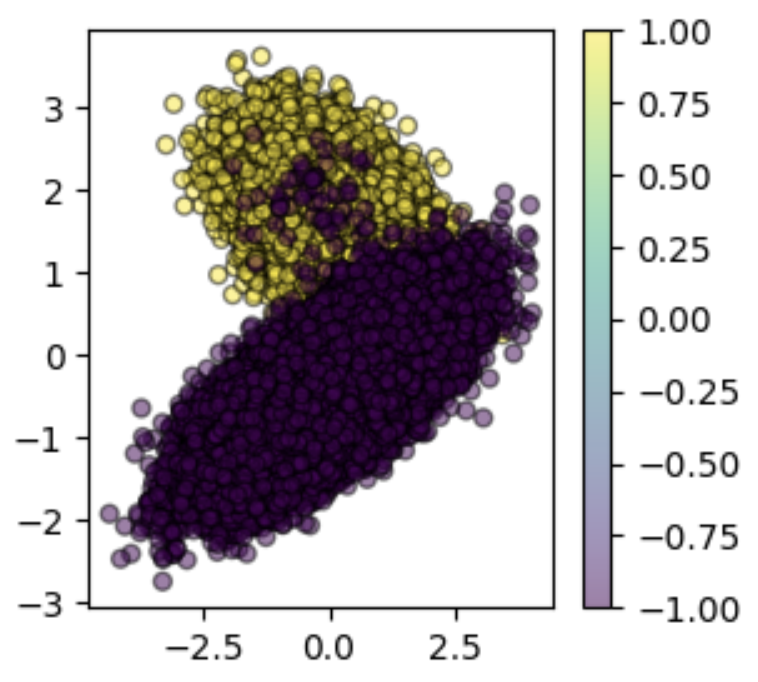
\includegraphics[width=\linewidth]{images/ds1.png}
        \caption{Train set 1.}
        \label{fig:ds1}
    \end{minipage}
    \hfill
    \begin{minipage}{0.49\textwidth}
        \centering
        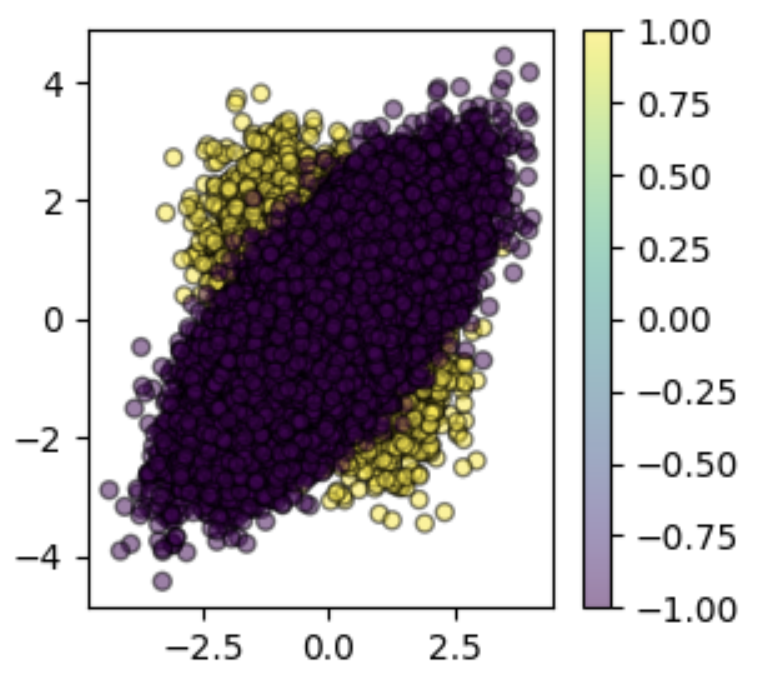
\includegraphics[width=\linewidth]{images/ds5.png}
        \caption{Train set 5.}
        \label{fig:ds5}
    \end{minipage}
\end{figure}

Di seguito, elenchiamo i valori di alcuni iperparametri rimasti immutati per tutti gli esperimenti. La simbologia adottata è la stessa rispetto ai Paragrafi \ref{par:primi-classificatori} e \ref{par:ultimo-classificatore}.
\begin{itemize}
    \item $C_+^{\text{min}} = 0.01, C_+^{\text{max}}=20$;

    \item $\Gamma$ contiene i valori da 0.1 a 50 con incrementi di 0.1;

    \item $H_{\text{min}} = 1, H_{\text{max}}=50$;

    \item $\sigma = 0.3z$;

    \item $F_{\text{min}} = 1$.
\end{itemize}











\subsection{SVM}
\label{par:svm-results}

Le Tabelle \ref{tab:performance-ds1-svm}-\ref{tab:performance-ds5-svm} illustrano le performance di vari FLF, addestrati usando SVM lineari, sui dataset considerati. In ciascuna tabella le colonne, in ordine, sono:
\begin{itemize}
    \item la lunghezza massima della catena ($t$),
    \item il FPR richiesto ($\bar \epsilon$),
    \item il numero di classificatori effettivamente impiegati,
    \item il FPR empirico raggiunto sul test set,
    \item il rapporto, in percentuale, tra lo spazio occupato dalla catena e quello occupato da un BF classico che gestisce lo stesso numero di chiavi con lo stesso FPR empirico.
\end{itemize}
In ogni tabella, ciascuna riga si riferisce a una specifica combinazione di $t$ e $\bar \epsilon$, che sono iperparametri. Il segno * indica che, per la relativa combinazione di $t$ e $\bar \epsilon$, l'addestramento ha portato ad avere solo un DT, senza alcuna SVM prima di esso.

È importante precisare che in nessun caso utilizzare un albero di decisione come ultimo classificatore della catena è stato conveniente rispetto a impiegare un BF classico.












La Tabella \ref{tab:svm-skip} prende in considerazione una singola catena avente $t=20$ e $\bar\epsilon=0.1$ e illustra l'andamento di alcuni dati rilevanti al proseguire delle iterazioni (indicizzate con $j$) durante l'addestramento di un FLF sul dataset 1, quello più semplice. I dati riportati sono:
\begin{itemize}
\item le chiavi rimaste al termine dell'iterazione $j$-esima,
\item le non-chiavi rimaste al termine dell'iterazione $j$-esima,
\item il FPR empirico del classificatore $j$-esimo,
\item il valore di $z$ per il classificatore $j$-esimo,
\item lo spazio, in bit, occupato dal classificatore $j$-esimo,
\item il rapporto, in percentuale, tra lo spazio occupato dal classificatore e quello occupato dal BF classico equivalente (indicato con $\rho$).
\end{itemize}

La Tabella \ref{tab:svm-no-skip} è analoga alla Tabella \ref{tab:svm-skip}, ma riguarda un setting in cui non è possibile effettuare salti all'ultimo classificatore, permettendo l'aggiunta anche di modelli sconvenienti dal punto di vista dello spazio.















\subsection{NN}

Le Tabelle \ref{tab:performance-ds1-mlp}-\ref{tab:performance-ds5-mlp} sono analoghe a quelle del Paragrafo \ref{par:svm-results}, ma si riferiscono a uno scenario in cui il FLF impiega NN al posto di SVM lineari.
Anche in questo caso, utilizzare un albero di decisione come ultimo classificatore della catena è sempre stato sconveniente rispetto a impiegare un BF classico.
Le Tabelle \ref{tab:mlp-skip} e \ref{tab:mlp-no-skip} sono rispettivamente analoghe alle Tabelle \ref{tab:svm-skip} e \ref{tab:svm-no-skip}, ma riguardano FLF che utilizzano NN.
















\subsection{Osservazioni}

Innanzitutto, è importante evidenziare che in nessun caso è stato conveniente utilizzare un DT come ultimo classificatore. Ciò significa che nessuno dei filtri ottenuti è puramente appreso; al contrario, ciascuno adotta un BF classico. Molto probabilmente questo è dovuto al fatto che, come osservato nel Paragrafo \ref{par:ultima-iterazione}, al progredire delle iterazioni, le chiavi che rimangono sono quelle più difficili da identificare, per cui il vantaggio di un modello di ML rispetto a un BF classico si fa via via più sottile. All'ultima iterazione, evidentemente, rimangono solo chiavi che non seguono alcun pattern, e dunque sfruttare un modello di ML perde di senso.

È da sottolineare anche il fatto che, fissato un $\bar \epsilon$, all'aumentare di $t$ l'efficienza tende, nella maggior parte dei casi, a peggiorare. Solitamente, i risultati migliori si hanno per $t=2$.

Tuttavia, nel complesso, un filtro basato su NN è quasi sempre più efficiente rispetto all'equivalente BF classico. Come ci sarebbe potuto aspettare, il vantaggio di questo tipo di filtro è minore su dataset in cui molte chiavi sono sovrapposte alle non-chiavi. Infatti, maggiore la sovrapposizione dei cluster di positivi e di negativi, maggiore è il rapporto tra lo spazio occupato dal filtro e da un BF classico. Sui dataset 4 e 5, per diverse combinazioni di $t$ e $\bar \epsilon$, tale rapporto arriva a essere maggiore di 1.

Confrontando i FLF basati su SVM con quelli basati su NN, notiamo che questi ultimi tendono a essere più efficienti, specialmente all'aumentare della difficoltà del dataset.
È importante sottolineare, però, che abbiamo considerato solo dataset formati da un cluster per classe; se ce ne fossero stati ulteriori, il problema sarebbe stato meno lineare e dunque più difficile per le SVM lineari.

Sul dataset 5, con i FLF basati su SVM, emerge un comportamento del filtro che differisce da quello osservato sui dataset precedenti. Data la grande difficoltà del dataset, se $t$ supera un certo valore, la seconda SVM non riesce a raggiungere il FPR richiesto (che diventa più stringente all'aumentare di $t$); dunque, si salta all'ultimo classificatore, il BF classico, dopo una sola iterazione. Si ottiene quindi un filtro composto da una SVM, che riconosce pochi positivi, e da un BF classico che gestisce i restanti, ossia la quasi totalità delle chiavi. Per questo, i filtri così generati hanno dimensioni molto simili rispetto ai BF classici equivalenti.

Esaminando le tabelle che illustrano la progressione delle iterazioni di un singolo filtro, possiamo chiaramente notare l'impatto sull'efficienza della possibilità di effettuare il salto all'ultimo classificatore. 
Notiamo anche che $\rho$ tende ad aumentare nel corso delle iterazioni, con diminuzioni occasionali probabilmente dovute al fatto che alcuni modelli, commettendo FP, rimuovono anche alcune non-chiavi che ostacolavano particolarmente l'identificazione dei positivi.
È interessante notare anche che, nel caso del filtro basato su NN con possibilità di salto, le singole NN non hanno mai raggiunto grandi dimensioni; anzi, si sono mantenute tutte sulla dimensione minima (corrispondente a 1 neurone per strato nascosto). Quindi, anche con NN così piccole si può raggiungere il FPR accettabile.

\begin{table}
    \centering
    \begin{tabular}{|c|c|c|c|c|}
        \hline
        $t$ & $\bar\epsilon$ & Classificatori usati & $\epsilon$ empirico & Spazio rispetto a BF \\ 
        \hline
        2 & 0.1 & 2 & 0.109 & 3.13\% \\  
        3 & 0.1 & 3 & 0.105 & 3.44\% \\  
        4 & 0.1 & 4 & 0.106 & 3.75\% \\  
        5 & 0.1 & 5 & 0.104 & 4.07\% \\  
        10 & 0.1 & 8 & 0.107 & 4.00\% \\ 
        20 & 0.1 & 13 & 0.099 & 4.40\% \\ 
        50 & 0.1 & 22 & 0.101 & 5.20\% \\ 
        100 & 0.1 & * & * & * \\ 
        2 & 0.05 & 2 & 0.048 & 3.92\% \\  
        3 & 0.05 & 3 & 0.053 & 3.98\% \\  
        4 & 0.05 & 4 & 0.054 & 4.09\% \\  
        5 & 0.05 & 5 & 0.054 & 4.32\% \\  
        10 & 0.05 & 10 & 0.055 & 5.13\% \\ 
        20 & 0.05 & 19 & 0.056 & 5.79\% \\ 
        50 & 0.05 & * & * & * \\ 
        100 & 0.05 & * & * & * \\  
        \hline
    \end{tabular}
    \caption{Performance del filtro basato su SVM sul dataset 1.}
    \label{tab:performance-ds1-svm}
\end{table}
\begin{table}
    \centering
    \begin{tabular}{|c|c|c|c|c|}
        \hline
        $t$ & $\bar\epsilon$ & Classificatori usati & $\epsilon$ empirico & Spazio rispetto a BF \\ 
        \hline
        2  & 0.1  & 2  & 0.102 & 14.99\% \\  
        3  & 0.1  & 3  & 0.106 & 15.86\% \\  
        4  & 0.1  & 4  & 0.103 & 16.17\% \\  
        5  & 0.1  & 5  & 0.103 & 16.86\% \\  
        10 & 0.1  & 10 & 0.104 & 19.10\% \\ 
        20 & 0.1  & 20 & 0.102 & 22.32\% \\ 
        50 & 0.1  & 50 & 0.104 & 28.18\% \\ 
        100 & 0.1 & 82 & 0.103 & 24.80\% \\  
        2  & 0.05 & 2  & 0.050 & 20.32\% \\  
        3  & 0.05 & 3  & 0.052 & 21.24\% \\  
        4  & 0.05 & 4  & 0.051 & 21.74\% \\  
        5  & 0.05 & 5  & 0.052 & 22.62\% \\  
        10 & 0.05 & 10 & 0.054 & 25.17\% \\ 
        20 & 0.05 & 20 & 0.053 & 28.86\% \\ 
        50 & 0.05 & 50 & 0.054 & 34.42\% \\ 
        100 & 0.05 & *  & *     & *      \\  
        \hline
    \end{tabular}
    \caption{Performance del filtro basato su SVM sul dataset 2.}
    \label{tab:performance-ds2-svm}
\end{table}
\begin{table}
    \centering
    \begin{tabular}{|c|c|c|c|c|}
        \hline
        $t$ & $\bar\epsilon$ & Classificatori usati & $\epsilon$ empirico & Spazio rispetto a BF \\ 
        \hline
        2  & 0.1  & 2  & 0.102 & 62.29\% \\  
        3  & 0.1  & 3  & 0.107 & 73.57\% \\  
        4  & 0.1  & 4  & 0.106 & 79.50\% \\  
        5  & 0.1  & 5  & 0.104 & 83.96\% \\  
        10 & 0.1  & 10 & 0.105 & 97.19\% \\ 
        20 & 0.1  & 20 & 0.105 & 112.48\% \\ 
        50 & 0.1  & 50 & 0.104 & 135.49\% \\ 
        100 & 0.1 & 51 & 0.105 & 76.90\% \\  
        2  & 0.05 & 2  & 0.053 & 68.94\% \\  
        3  & 0.05 & 3  & 0.055 & 78.91\% \\  
        4  & 0.05 & 4  & 0.054 & 83.89\% \\  
        5  & 0.05 & 5  & 0.053 & 87.94\% \\  
        10 & 0.05 & 10 & 0.053 & 100.69\% \\ 
        20 & 0.05 & 20 & 0.053 & 112.59\% \\ 
        50 & 0.05 & 50 & 0.053 & 132.77\% \\ 
        100 & 0.05 & 39 & 0.052 & 77.14\% \\  
        \hline
    \end{tabular}
    \caption{Performance del filtro basato su SVM sul dataset 3.}
    \label{tab:performance-ds3-svm}
\end{table}
\begin{table}
    \centering
    \begin{tabular}{|c|c|c|c|c|}
        \hline
        $t$ & $\bar\epsilon$ & Classificatori usati & $\epsilon$ empirico & Spazio rispetto a BF \\ 
        \hline
        2  & 0.1  & 2  & 0.101 & 85.31\% \\  
        3  & 0.1  & 3  & 0.108 & 101.83\% \\  
        4  & 0.1  & 4  & 0.104 & 112.89\% \\  
        5  & 0.1  & 5  & 0.106 & 120.41\% \\  
        10 & 0.1  & 10 & 0.104 & 143.40\% \\ 
        20 & 0.1  & 20 & 0.103 & 165.85\% \\ 
        50 & 0.1  & 50 & 0.104 & 195.58\% \\ 
        100 & 0.1 & 20 & 0.103 & 90.63\% \\  
        2  & 0.05 & 2  & 0.051 & 89.88\% \\  
        3  & 0.05 & 3  & 0.052 & 103.12\% \\  
        4  & 0.05 & 4  & 0.053 & 112.02\% \\  
        5  & 0.05 & 5  & 0.052 & 118.67\% \\  
        10 & 0.05 & 10 & 0.054 & 135.93\% \\ 
        20 & 0.05 & 20 & 0.053 & 155.21\% \\ 
        50 & 0.05 & 28 & 0.052 & 102.28\% \\ 
        100 & 0.05 & 13 & 0.050 & 91.15\% \\  
        \hline
    \end{tabular}
    \caption{Performance del filtro basato su SVM sul dataset 4.}
    \label{tab:performance-ds4-svm}
\end{table}
\begin{table}
    \centering
    \begin{tabular}{|c|c|c|c|c|}
        \hline
        $t$ & $\bar\epsilon$ & Classificatori usati & $\epsilon$ empirico & Spazio rispetto a BF \\ 
        \hline
        2  & 0.1  & 2  & 0.107 & 106.23\% \\  
        3  & 0.1  & 3  & 0.104 & 125.15\% \\  
        4  & 0.1  & 4  & 0.101 & 138.85\% \\  
        5  & 0.1  & 2  & 0.098 & 97.27\% \\  
        10 & 0.1  & 2  & 0.104 & 96.11\% \\ 
        20 & 0.1  & 2  & 0.098 & 96.13\% \\ 
        50 & 0.1  & 2  & 0.100 & 96.58\% \\ 
        100 & 0.1 & 2  & 0.105 & 97.06\% \\  
        2  & 0.05 & 2  & 0.052 & 107.82\% \\  
        3  & 0.05 & 2  & 0.049 & 102.24\% \\  
        4  & 0.05 & 2  & 0.050 & 99.98\% \\  
        5  & 0.05 & 2  & 0.052 & 98.98\% \\  
        10 & 0.05 & 2  & 0.049 & 97.40\% \\ 
        20 & 0.05 & 2  & 0.050 & 97.16\% \\ 
        50 & 0.05 & 2  & 0.049 & 97.30\% \\ 
        100 & 0.05 & 2  & 0.051 & 97.95\% \\  
        \hline
    \end{tabular}
    \caption{Performance del filtro basato su SVM sul dataset 5.}
    \label{tab:performance-ds5-svm}
\end{table}
\begin{table}
\centering
\begin{tabular}{|c|c|c|c|c|c|c|}
\hline
$j$ & Chiavi & Non-chiavi & $\epsilon_i \cdot 10^2$ & $z_i \cdot 10^2$ & Spazio [bit] & $\rho$ [\%] \\
\hline
1 & 1198 & 55495 & 0.5269 & 0.5254 & 96 & 0.05 \\
2 & 935 & 55219 & 0.5213 & 0.5253 & 96 & 3.34 \\
3 & 785 & 54929 & 0.5240 & 0.5256 & 96 & 5.85 \\
4 & 696 & 54642 & 0.5268 & 0.5257 & 96 & 9.88 \\
5 & 634 & 54380 & 0.5211 & 0.5256 & 96 & 14.14 \\
6 & 591 & 54042 & 0.5324 & 0.5259 & 96 & 20.47 \\
7 & 545 & 53739 & 0.5180 & 0.5254 & 96 & 19.05 \\
8 & 524 & 53372 & 0.5380 & 0.5260 & 96 & 41.92 \\
9 & 508 & 53111 & 0.5235 & 0.5250 & 96 & 54.86 \\
10 & 495 & 52813 & 0.5262 & 0.5251 & 96 & 67.61 \\
11 & 484 & 52557 & 0.5290 & 0.5250 & 96 & 79.34 \\
12 & 471 & 52323 & 0.5230 & 0.5246 & 96 & 67.13 \\
13 & 0 & 50260 & 4.072 & 4.122 & 3126 & (100) \\
\hline
\end{tabular}
\caption{Progressione delle iterazioni utilizzando SVM lineari e con la possibilità di salto. FPR empirico: 0.099; spazio rispetto a un BF equivalente: 4.40\%.}
\label{tab:svm-skip}
\end{table}
\begin{table}
\centering
\begin{tabular}{|c|c|c|c|c|c|c|}
\hline
$j$ & Chiavi & Non-chiavi & $\epsilon_i \cdot 10^3$ & $z_i \cdot 10^3$ & Spazio [bit] & $\rho$ [\%] \\
\hline
1  & 1198  & 55495 & 5.269 & 5.254 & 96   & 0.05 \\
2  & 935   & 55219 & 5.213 & 5.253 & 96   & 3.34 \\
3  & 785   & 54929 & 5.240 & 5.256 & 96   & 5.85 \\
4  & 696   & 54642 & 5.268 & 5.257 & 96   & 9.88 \\
5  & 634   & 54380 & 5.211 & 5.256 & 96   & 14.14 \\
6  & 591   & 54042 & 5.324 & 5.259 & 96   & 20.47 \\
7  & 545   & 53739 & 5.180 & 5.254 & 96   & 19.05 \\
8  & 524   & 53372 & 5.380 & 5.260 & 96   & 41.92 \\
9  & 508   & 53111 & 5.235 & 5.250 & 96   & 54.86 \\
10 & 495   & 52813 & 5.262 & 5.251 & 96   & 67.61 \\
11 & 484   & 52557 & 5.290 & 5.250 & 96   & 79.34 \\
12 & 471   & 52323 & 5.230 & 5.246 & 96   & 67.13 \\
13 & 464   & 52081 & 5.168 & 5.248 & 96   & 124.68 \\
14 & 455   & 51768 & 5.195 & 5.259 & 96   & 96.97 \\
15 & 439   & 51483 & 5.222 & 5.270 & 96   & 54.86 \\
16 & 434   & 51238 & 5.249 & 5.279 & 96   & 174.55 \\
17 & 430   & 50965 & 5.277 & 5.287 & 96   & 218.18 \\
18 & 421   & 50620 & 5.214 & 5.290 & 96   & 96.97 \\
19 & 418   & 50367 & 5.241 & 5.329 & 96   & 290.91 \\
20 & 0     & 50052 & 6.008 & 5.416 & 4540 & (100) \\
\hline
\end{tabular}
\caption{Progressione delle iterazioni utilizzando SVM lineari e senza la possibilità di salto. FPR empirico: 0.103; spazio rispetto a un BF equivalente: 65.42\%.}
\label{tab:svm-no-skip}
\end{table}
\begin{table}
    \centering
    \begin{tabular}{|c|c|c|c|c|}
        \hline
        $t$  & $\bar\epsilon$ & Classificatori usati & $\epsilon$ empirico & Spazio rispetto a BF \\ 
        \hline
        2   & 0.1  & 2  & 0.103 & 3.31\% \\ 
        3   & 0.1  & 3  & 0.105 & 3.70\% \\ 
        4   & 0.1  & 4  & 0.103 & 4.20\% \\ 
        5   & 0.1  & 5  & 0.103 & 4.65\% \\  
        10  & 0.1  & 6  & 0.107 & 4.39\% \\  
        20  & 0.1  & 9  & 0.103 & 4.97\% \\  
        2   & 0.05 & 2  & 0.050 & 4.02\% \\ 
        3   & 0.05 & 3  & 0.056 & 4.17\% \\ 
        4   & 0.05 & 4  & 0.053 & 4.39\% \\ 
        5   & 0.05 & 5  & 0.054 & 4.72\% \\  
        10  & 0.05 & 8  & 0.049 & 5.21\% \\  
        20  & 0.05 & 10 & 0.054 & 5.50\% \\  
        \hline
    \end{tabular}
    \caption{Performance del filtro basato su NN sul dataset 1.}
    \label{tab:performance-ds1-mlp}
\end{table}
\begin{table}
    \centering
    \begin{tabular}{|c|c|c|c|c|}
        \hline
        $t$  & $\bar\epsilon$ & Classificatori usati & $\epsilon$ empirico & Spazio rispetto a BF \\ 
        \hline
        2   & 0.1  & 2  & 0.100 & 15.11\% \\ 
        3   & 0.1  & 3  & 0.106 & 16.66\% \\ 
        4   & 0.1  & 4  & 0.103 & 16.72\% \\ 
        5   & 0.1  & 5  & 0.104 & 17.43\% \\  
        10  & 0.1  & 10 & 0.102 & 20.78\% \\  
        20  & 0.1  & 20 & 0.105 & 26.58\% \\  
        2   & 0.05 & 2  & 0.049 & 20.39\% \\ 
        3   & 0.05 & 3  & 0.051 & 22.24\% \\ 
        4   & 0.05 & 4  & 0.052 & 22.12\% \\ 
        5   & 0.05 & 5  & 0.052 & 23.28\% \\  
        10  & 0.05 & 10 & 0.052 & 24.82\% \\  
        20  & 0.05 & 20 & 0.052 & 29.77\% \\  
        \hline
    \end{tabular}
    \caption{Performance del filtro basato su NN sul dataset 2.}
    \label{tab:performance-ds2-mlp}
\end{table}
\begin{table}
    \centering
    \begin{tabular}{|c|c|c|c|c|}
        \hline
        $t$  & $\bar\epsilon$ & Classificatori usati & $\epsilon$ empirico & Spazio rispetto a BF \\ 
        \hline
        2   & 0.1  & 2  & 0.106 & 62.68\% \\ 
        3   & 0.1  & 3  & 0.105 & 61.95\% \\ 
        4   & 0.1  & 4  & 0.098 & 63.90\% \\ 
        5   & 0.1  & 5  & 0.100 & 66.16\% \\  
        10  & 0.1  & 10 & 0.100 & 75.80\% \\  
        20  & 0.1  & 20 & 0.101 & 90.13\% \\  
        2   & 0.05 & 2  & 0.047 & 69.57\% \\ 
        3   & 0.05 & 3  & 0.049 & 68.86\% \\ 
        4   & 0.05 & 4  & 0.049 & 70.65\% \\ 
        5   & 0.05 & 5  & 0.050 & 73.69\% \\  
        10  & 0.05 & 10 & 0.049 & 85.20\% \\  
        20  & 0.05 & 20 & 0.049 & 94.67\% \\  
        \hline
    \end{tabular}
    \caption{Performance del filtro basato su NN sul dataset 3.}
    \label{tab:performance-ds3-mlp}
\end{table}
\begin{table}
    \centering
    \begin{tabular}{|c|c|c|c|c|}
        \hline
        $t$  & $\bar\epsilon$ & Classificatori usati & $\epsilon$ empirico & Spazio rispetto a BF \\ 
        \hline
        2   & 0.1  & 2  & 0.099 & 77.00\% \\ 
        3   & 0.1  & 3  & 0.099 & 83.31\% \\ 
        4   & 0.1  & 4  & 0.094 & 87.23\% \\ 
        5   & 0.1  & 5  & 0.098 & 92.26\% \\  
        10  & 0.1  & 10 & 0.098 & 108.26\% \\  
        20  & 0.1  & 20 & 0.097 & 123.45\% \\  
        2   & 0.05 & 2  & 0.052 & 81.85\% \\ 
        3   & 0.05 & 3  & 0.050 & 87.74\% \\ 
        4   & 0.05 & 4  & 0.049 & 92.05\% \\ 
        5   & 0.05 & 5  & 0.048 & 96.27\% \\  
        10  & 0.05 & 10 & 0.049 & 106.96\% \\  
        20  & 0.05 & 20 & 0.049 & 128.04\% \\  
        \hline
    \end{tabular}
    \caption{Performance del filtro basato su NN sul dataset 4.}
    \label{tab:performance-ds4-mlp}
\end{table}
\begin{table}
    \centering
    \begin{tabular}{|c|c|c|c|c|}
        \hline
        $t$  & $\bar\epsilon$ & Classificatori usati & $\epsilon$ empirico & Spazio rispetto a BF \\ 
        \hline
        2   & 0.1  & 2  & 0.095 & 95.15\% \\ 
        3   & 0.1  & 3  & 0.100 & 104.46\% \\ 
        4   & 0.1  & 4  & 0.096 & 111.72\% \\ 
        5   & 0.1  & 5  & 0.097 & 117.78\% \\  
        10  & 0.1  & 10 & 0.098 & 143.04\% \\  
        20  & 0.1  & 20 & 0.093 & 152.17\% \\  
        2   & 0.05 & 2  & 0.053 & 97.09\% \\ 
        3   & 0.05 & 3  & 0.050 & 106.45\% \\ 
        4   & 0.05 & 4  & 0.050 & 111.99\% \\ 
        5   & 0.05 & 5  & 0.050 & 117.11\% \\  
        10  & 0.05 & 10 & 0.046 & 127.85\% \\  
        20  & 0.05 & 20 & 0.047 & 147.61\% \\  
        \hline
    \end{tabular}
    \caption{Performance del filtro basato su NN sul dataset 5.}
    \label{tab:performance-ds5-mlp}
\end{table}
\begin{table}
\centering
\begin{tabular}{|c|c|c|c|c|c|c|}
\hline
$j$ & Chiavi & Non-chiavi & $\epsilon_i \cdot 10^3$ & $z_i \cdot 10^3$ & Spazio [bit] & $\rho$ [\%] \\
\hline
1 & 1201 & 55495 & 5.269 & 5.254 & 224 & 0.11 \\
2 & 931 & 55216 & 5.297 & 5.253 & 224 & 7.60 \\
3 & 783 & 54910 & 5.241 & 5.251 & 224 & 13.84 \\
4 & 698 & 54636 & 5.184 & 5.252 & 224 & 24.06 \\
5 & 636 & 54379 & 5.211 & 5.256 & 224 & 32.99 \\
6 & 599 & 54050 & 5.324 & 5.259 & 224 & 55.45 \\
7 & 552 & 53700 & 5.266 & 5.254 & 224 & 43.58 \\
8 & 524 & 53383 & 5.207 & 5.253 & 224 & 72.96 \\
9 & 0 & 50327 & 60.02 & 61.29 & 3045 & (100) \\
\hline
\end{tabular}
\caption{Progressione delle iterazioni utilizzando NN e con la possibilità di salto. FPR empirico: 0.103; spazio rispetto a un BF equivalente: 4.97\%.}
\label{tab:mlp-skip}
\end{table}
\begin{table}
\centering
\begin{tabular}{|c|c|c|c|c|c|c|}
\hline
$j$ & Chiavi & Non-chiavi & $\epsilon_i \cdot 10^3$ & $z_i \cdot 10^3$ & Spazio [bit] & $\rho$ [\%] \\
\hline
1  & 1201  & 55495 & 5.269 & 5.254 & 224  & 0.11 \\
2  & 931   & 55216 & 5.297 & 5.253 & 224  & 7.60 \\
3  & 783   & 54910 & 5.241 & 5.251 & 224  & 13.84 \\
4  & 698   & 54636 & 5.184 & 5.252 & 224  & 24.06 \\
5  & 636   & 54379 & 5.211 & 5.256 & 224  & 32.99 \\
6  & 599   & 54050 & 5.324 & 5.259 & 224  & 55.45 \\
7  & 552   & 53700 & 5.266 & 5.254 & 224  & 43.58 \\
8  & 524   & 53383 & 5.207 & 5.253 & 224  & 72.96 \\
9  & 494   & 53142 & 5.321 & 5.257 & 480  & 146.79 \\
10 & 474   & 52864 & 5.175 & 5.251 & 1184 & 538.18 \\
11 & 470   & 52644 & 5.113 & 5.259 & 1632 & 3709.09 \\
12 & 460   & 52284 & 5.140 & 5.275 & 480  & 436.36 \\
13 & 448   & 51980 & 5.166 & 5.292 & 1184 & 896.97 \\
14 & 438   & 51739 & 5.014 & 5.310 & 1184 & 1066.67 \\
15 & 430   & 51450 & 4.949 & 5.359 & 1184 & 1330.34 \\
16 & 422   & 51097 & 6.421 & 5.441 & 1184 & 1392.94 \\
17 & 420   & 50923 & 3.641 & 5.196 & 1184 & 4933.33 \\
18 & 417   & 50573 & 5.938 & 5.715 & 1632 & 4945.45 \\
19 & 414   & 50357 & 5.054 & 5.603 & 1632 & 4800.00 \\
20 & 0    & 50037 & 7.389 & 6.151 & 4386 & (100) \\
\hline
\end{tabular}
\caption{Progressione delle iterazioni utilizzando NN e senza la possibilità di salto. FPR empirico: 0.103; spazio rispetto a un BF equivalente: 19.67\%.}
\label{tab:mlp-no-skip}
\end{table}
\chapter{Conclusioni}

Abbiamo sperimentato con un approccio puramente appreso per il problema dell'approximate set membership, con l'obiettivo di giungere a un filtro di Bloom composto interamente da modelli di machine learning, come possibile alternativa più efficiente rispetto ai filtri di Bloom classici e a quelli parzialmente appresi. In particolare, abbiamo sviluppato un filtro configurato come una sequenza di classificatori. In una prima variante, tale sequenza è composta da support vector machine lineari, seguite da un albero di decisione finale; nella seconda variante, invece, abbiamo reti neurali, anch'esse seguite da un albero di decisione. 

Dopo aver misurato su alcuni insiemi di dati le prestazioni di diversi filtri puramente appresi, abbiamo osservato che, in genere, questo approccio conviene rispetto a quello classico, non appreso, ma non conviene rispetto a quello parzialmente appreso. 
In ogni esperimento condotto, utilizzare una catena composta interamente da modelli di machine learning non è stato vantaggioso rispetto a una avente al suo termine un filtro di Bloom classico. Inoltre, all'aumentare della lunghezza della sequenza, abbiamo riscontrato un peggioramento dell'efficienza in termini di spazio occupato. 
Tuttavia, anche se la sequenza di modelli ottimale non è puramente appresa, siamo giunti a un approccio innovativo per aggiungere, controllare e dimensionare i singoli classificatori che la compongono. Ulteriori sperimentazioni, ad esempio sfruttando altre tipologie di modello, potrebbero portare a nuovi interessanti risultati. 

\printbibliography

\end{document}